\subsection{Mac Lane's separability criterion}

THEOREM 1. --- Let K be a field of characteristic 0. Every reduced K-algebra and in particular every extension of K is separable over K.

We first show that every extension L of K is separable. Let B be a transcendence basis of L over K (V, p.~109, Th. 1) and let \(L_{1} = \mathbf{K}(\mathbf{B})\) . Then \(L_{1}\) is separable over K (V, p.~121, Prop. 6). Further, L is an algebraic extension of \(L_{1}\) and \(L_{1}\) is a field of characteristic 0; therefore L is separable over \(L_{1}\) (V, p.~37, Cor.). By Prop. 9, L is thus separable over K.

Now let A be a reduced algebra over the field K. By the Cor. of Prop. 2 (V, p.~119) there exists a family \((L_{i})_{i \in I}\) of extensions of K such that A is isomorphic to a subalgebra of \(\prod_{i \in I} L_{i}\) . Each of the algebras \(L_{i}\) is separable over K by what has

been said and so A has the same property, by Prop. 3 a) and c) (V, p.~119).

THEOREM 2. --- Let K be a field of characteristic \(p \neq 0\) , \(\mathbf{K}^{p^{-\infty}}\) a perfect closure of K and A a commutative K-algebra. The following properties are equivalent:

\begin{enumerate}
\def\labelenumi{\alph{enumi})}
\item
  A is separable.
\item
  There exists an extension \(\mathbf{K}'\) of \(\mathbf{K}\) such that \(\mathbf{K}'\) is perfect and \(\mathbf{K}' \otimes_{\mathbf{K}} \mathbf{A}\) is reduced.
\item
  The ring \(\mathbf{K}^{p^{-\infty}}\otimes_{\mathbf{K}}\mathbf{A}\) is reduced.
\item
  The ring \(\mathbf{K}' \otimes_{\mathbf{K}} \mathbf{A}\) is reduced for every extension \(\mathbf{K}'\) of \(\mathbf{K}\) which is of finite degree and \(p\) -radical of height \(\leqslant 1\) .
\item
  For every family \((a_{i})_{i\in I}\) of elements of A linearly free over K, the family \((a_{i}^{p})_{i\in I}\) is linearly free over K.
\item
  There exists a basis \((a_{i})_{i\in I}\) of the vector K-space A such that the family \((a_{i}^{p})_{i\in I}\) is linearly free over K.
\end{enumerate}

If an extension \(\mathbf{K}'\) of \(\mathbf{K}\) is a perfect field, it contains a subextension \(\mathbf{K}\) -isomorphic to \(\mathbf{K}^{p^{-\infty}}\) (V, p.~6, Prop. 3); moreover, every \(p\) -radical extension of \(\mathbf{K}\) is isomorphic to a subextension of \(\mathbf{K}^{p^{-\infty}}\) (V, p.~26, Prop. 3). These remarks show the implications \(a) \Rightarrow b) \Rightarrow c) \Rightarrow d)\) .

Let us prove that \(d)\) implies \(e)\) . Let \((a_i)_{i \in I}\) be a linearly free family in \(A\) and let \((\lambda_i)_{i \in I}\) be a family of finite support in \(K\) such that \(\sum \lambda_i a_i^p = 0\) . Let \(K'\) be the subextension of \(K^{p^{-\infty}}\) generated by the elements \(\lambda_i^{p^{-1}}\) ; it is of finite degree and height \(\leqslant 1\) . Put \(x = \sum_{i \in I} \lambda_i^{p^{-1}} \otimes a_i\) in \(K' \otimes_K A\) ; we have

\[
x ^ {p} = \sum_ {i \in I} \lambda_ {i} \otimes a _ {i} ^ {p} = 1 \otimes \sum_ {i \in I} \lambda_ {i} a _ {i} ^ {p} = 0.
\]

By the hypothesis \(d)\) we have \(x = 0\) , whence \(\lambda_i = 0\) for all \(i \in I\) .

Clearly \(e)\) implies \(f)\) and it remains to show that \(f)\) implies \(a)\) . Thus let \((a_i)_{i \in I}\) be a basis of \(A\) over \(K\) such that the family \((a_i^p)_{i \in I}\) is linearly free over \(K\) . Let \(L\) be an extension of \(K\) and let \(x\) be an element of \(L \otimes_K A\) such that \(x^p = 0\) . Write \(x = \sum_{i \in I} \lambda_i \otimes a_i\) with \(\lambda_i \in L\) for all \(i \in I\) . We have \(x^p =\)

\(\sum_{i\in I}\lambda_i^p\otimes a_i^p = 0\) and since the family \((a_i^p)_{i\in I}\) is linearly free over \(\mathbf{K}\) , we have

\(\lambda_{i}^{p} = 0\) , whence \(\lambda_{i} = 0\) for all \(i \in I\) ; it follows that \(x = 0\) . So we have proved that \(x^{p} = 0\) implies \(x = 0\) in \(\mathbf{L} \otimes_{\mathbf{K}} \mathbf{A}\) , from which it follows at once that \(\mathbf{L} \otimes_{\mathbf{K}} \mathbf{A}\) is reduced.

COROLLARY 1 (Mac Lane). --- Let K be a field of characteristic exponent p, Ω a perfect extension of K and L a subextension of Ω. Then the following conditions are equivalent :

\begin{enumerate}
\def\labelenumi{\alph{enumi})}
\item
  L is separable over K.
\item
  L is linearly disjoint from \(\mathbf{K}^{p^{-\infty}}\) over \(\mathbf{K}\) .
\item
  L is linearly disjoint over K from every p-radical extension of K contained in \(\Omega\) , of finite degree and height \(\leqslant 1\) .
\end{enumerate}

The case where K is of characteristic 0 is trivial because then L is separable over K (Th. 1) and \(K^{p^{-\infty}} = K\) by convention. Suppose then that \(p \neq 1\) , and let us first show that a) implies b). Assume that L is separable over K and let \((a_i)_{i \in I}\) be a basis of L over K. Let \((\lambda_i)_{i \in I}\) be a family of finite support of elements of \(K^{p^{-\infty}}\) such that \(\sum_{i \in I} \lambda_i a_i = 0\) ; there exists an integer \(f \geqslant 0\) and elements

\(\mu_{i}\) of \(\mathbf{K}\) such that \(\lambda_{i} = \mu_{i}^{p^{-f}}\) . We have

\[
\sum_ {i \in I} \mu_ {i} a _ {i} ^ {p ^ {f}} = \left(\sum_ {i \in I} \lambda_ {i} a _ {i}\right) ^ {p ^ {f}} = 0
\]

and Th. 2 implies, by induction on \(f\) , that the family \((a_i^{p^f})_{i\in I}\) is linearly free over \(K\) . We thus have \(\mu_i = 0\) , whence \(\lambda_i = 0\) for all \(i\in I\) . Finally \(L\) is linearly disjoint from \(K^{p^{-\infty}}\) over \(K\) .

It is clear that \(b)\) implies \(c)\) . Lastly suppose that \(c)\) holds and let \(K'\) be an extension of \(K\) of finite degree and \(p\) -radical of height \(\leqslant 1\) . The ring \(K' \otimes_K L\) is isomorphic to a subring of \(\Omega\) , hence is reduced. Now it follows from Th. 2 that \(L\) is separable over \(K\) .

COROLLARY 2. --- Let K be a field of characteristic exponent p, \(K^{p^{-\infty}}\) a perfect closure of K and L a separable extension of K. Then the ring \(L \otimes_{K} K^{p^{-\infty}}\) is a field. If moreover L is algebraic over K, then \(L \otimes_{K} K^{p^{-\infty}}\) is a perfect closure of L.

The case \(p = 1\) is trivial, so let us suppose \(p \neq 1\) . Let \(\Omega\) be a perfect closure of \(L\) . By Cor. 1 there exists a K-algebra homomorphism of \(L \otimes_K K^{p^{-\infty}}\) onto \(L[K^{p^{-\infty}}]\) which maps \(x \otimes y\) to \(xy\) for \(x \in L\) and \(y \in K^{p^{-\infty}}\) . Since \(K^{p^{-\infty}}\) is algebraic over \(K\) , the ring \(L[K^{p^{-\infty}}]\) is a subfield of \(\Omega\) (V, p.~18, Cor. 1). Suppose further that \(L\) is algebraic over \(K\) , then \(L[K^{p^{-\infty}}]\) is an algebraic extension of the perfect field \(K^{p^{-\infty}}\) , hence it is a perfect field (V, p.~43, Cor. 1); finally, since the field \(L[K^{p^{-\infty}}]\) is a \(p\) -radical extension of \(L\) (V, p.~25, Cor.), it is a perfect closure of \(L\) .

COROLLARY 3.--- Let L be an algebraic extension of K and M a commutative L-algebra (for example an extension of L). If M is separable over K, it is separable over L.

The algebra L is K-isomorphic to a subalgebra of M, hence L is a separable extension of K. Therefore (Cor. 2) there exists an L-isomorphism of \(L^{p^{-\infty}}\) onto \(K^{p^{-\infty}} \otimes_{K} L\) . The ring \(L^{p^{-\infty}} \otimes_{L} M\) is thus isomorphic to \((\mathrm{K}^{p^{-\infty}} \otimes_{K} L) \otimes_{L} M\) , and so to \(K^{p^{-\infty}} \otimes_{K} M\) (II, p.~278, Prop. 2) and this latter ring is reduced because M is separable over K. Thus the ring \(L^{p^{-\infty}} \otimes_{L} M\) is reduced, which proves that M is separable over L (V, p.~122, Th. 2).

Remark. --- Mac Lane's criterion may be formulated without introducing any extensions of K other than L. For by c) of Cor. 1, L is separable over K if and only if L and \(K^{p^{-1}}\) are linearly disjoint over K. Since the mapping \(x \mapsto x^{p}\) is an isomorphism of L onto the subfield \(L^{p}\) , we obtain the following criterion (cf.~V, p.~177, Ex. 11 for an analogous criterion for algebras):

L is separable over K if and only if the subfields \(L^{p}\) and K of L are linearly disjoint over \(K^{p}\) .

\subsection{Extensions of a perfect field}

For ease of reference we summarize the principal properties of extensions of perfect fields :

THEOREM 3. --- Let K be a perfect field.

\begin{enumerate}
\def\labelenumi{\alph{enumi})}
\item
  Every algebraic extension of \(\mathbf{K}\) is a perfect field.
\item
  Every extension of \(\mathbf{K}\) is separable.
\item
  For a K-algebra to be separable it is necessary and sufficient that it should be reduced.
\item
  Let \(\mathbf{A}\) and \(\mathbf{B}\) be two reduced K-algebras. Then \(\mathbf{A} \otimes_{\mathbf{K}} \mathbf{B}\) is reduced.
\item
  If \(\mathbf{E}\) and \(\mathbf{F}\) are two extensions of \(\mathbf{K}\) , then the ring \(\mathbf{E} \otimes_{\mathbf{K}} \mathbf{F}\) is reduced.
\end{enumerate}

Assertion \(a\) ) is just Cor. 1 of Prop. 11 (V, p.~43).

Assertion b) follows from Th. 1 (V, p.~122) when K is of characteristic 0 and from Cor. 1 (V, p.~123) when K is of characteristic \(p \neq 0\) .

Let us prove \(c\) ). The case where \(\mathbf{K}\) is of characteristic 0 follows from Th. 1 (V, p.~122). So it is enough to show that if \(\mathbf{K}\) is perfect of characteristic \(p \neq 0\) and \(\mathbf{A}\) is a reduced K-algebra, then \(\mathbf{A}\) is separable over \(\mathbf{K}\) . But this follows from the equivalence of the conditions \(a\) ) and \(b\) ) of Th. 2 (V, p.~122; take \(\mathbf{K}' = \mathbf{K}\) in \(b\) )).

Finally, \(d)\) follows from \(c)\) and Prop. 5 (V, p.~120) and \(e)\) is a particular case of \(d)\) .

\subsection{The characterization of separability by automorphisms}

THEOREM 4. --- Let \(\Omega\) be an algebraically closed extension of a field \(K\) and \(L\) a subextension of \(\Omega\) . Then the following conditions are equivalent:

\begin{enumerate}
\def\labelenumi{\alph{enumi})}
\item
  L is separable over K.
\item
  The intersection of the kernels of the \(\Omega\) -algebra homomorphisms of \(\Omega \otimes_{K} L\) into \(\Omega\) is reduced to 0.
\item
  For any elements \(a_1, \ldots, a_n\) of L linearly independent over K there exist K-automorphisms \(\sigma_1, \ldots, \sigma_n\) of \(\Omega\) such that \(\det(\sigma_i(a_j)) \neq 0\) .
\item
  Let V be a vector sub-K-space of L of finite dimension. Every K-linear mapping of V into \(\Omega\) is a linear combination (with coefficients in \(\Omega\) ) of the restrictions to V of K-automorphisms of \(\Omega\) .
\end{enumerate}

\(d) \Rightarrow c)\) : Let \(a_1, \ldots, a_n\) be elements of L linearly independent over K and let V be the vector sub-K-space of L generated by \(a_1, \ldots, a_n\) . The mapping \(f \mapsto (f(a_1), \ldots, f(a_n))\) is an \(\Omega\) -linear bijection of \(\mathrm{Hom}_{\mathbf{K}}(\mathbf{V}, \Omega)\) onto \(\Omega^n\) . Suppose that \(d)\) holds, then there exist K-automorphisms \(\sigma_1, \ldots, \sigma_n\) of \(\Omega\) such that the elements \((\sigma_i(a_1), \ldots, \sigma_i(a_n))\) of \(\Omega^n\) (for \(1 \leqslant i \leqslant n\) ) form a basis of \(\Omega^n\) . We thus have \(\det(\sigma_i(a_j)) \neq 0\) , so \(d)\) implies \(c)\) .

\(c) \Rightarrow b)\) : Assume that \(c)\) holds and let \(x\) be in \(\Omega \otimes_{\mathbb{K}} L\) . We write \(x\) in the form \(\sum_{j=1}^{n} x_j \otimes a_j\) with \(x_1, \ldots, x_n\) in \(\Omega\) and the elements \(a_1, \ldots, a_n\) of \(L\) linearly

independent over K. Choose K-automorphisms \(\sigma_{1},\ldots,\sigma_{n}\) of \(\Omega\) such that det \(\sigma_{i}(a_{j})\neq0\) ; let \(\chi_{1},\ldots,\chi_{n}\) be the \(\Omega\) -homomorphisms of \(\Omega\otimes_{K}L\) into \(\Omega\) such that \(\chi_{i}(a\otimes b)=a\cdot\sigma_{i}(b)\) for \(a\in\Omega\) and \(b\in L\) . Suppose that \(\chi_{i}(x)=0\) for \(1\leqslant i\leqslant n\) , in other words, that \(\sum_{j=1}^{n}x_{j}\cdot\sigma_{i}(a_{j})=0\) for \(1\leqslant i\leqslant n\) . Since we have assumed that the matrix \((\sigma_{i}(a_{j}))\) has a non-zero determinant, we have \(x_{i}=0\) for \(1\leqslant i\leqslant n\) and so \(x=0\) .

\(b) \Rightarrow a)\) : Since every extension of a field of characteristic 0 is separable (V, p.~122, Th. 1) it suffices to examine the case where K is of characteristic \(p \neq 0\) . Let X be the set of all \(\Omega\) -algebra homomorphisms of \(\Omega \otimes_{K} L\) into \(\Omega\) and \(f\) the homomorphism of \(\Omega \otimes_{K} L\) into \(\Omega^{X}\) defined by \(f(u) = (\chi(u))_{\chi \in X}\) for \(u \in \Omega \otimes_{K} L\) . Condition \(b)\) means that \(f\) is injective and so implies that the ring \(\Omega \otimes_{K} L\) is reduced. Hence condition \(b)\) of Th. 2 (V, p.~122) is satisfied with \(K' = \Omega\) , so L is separable over K.

\(a) \Rightarrow d)\) : Suppose that L is separable over K. Let V be a vector sub-K-space of finite dimension of L, \(V_{(\Omega)} = \Omega \otimes_K V\) the vector \(\Omega\) -space derived from V by extension of scalars and \(f_0\) the linear form on \(V_{(\Omega)}\) such that \(f_0(x \otimes y) = xy\) for \(x \in \Omega\) , \(y \in V\) . Denote by G the group of K-automorphisms of \(\Omega\) ; for \(\sigma \in G\) we put \(\sigma_V = \sigma \otimes Id_V\) and \(g_\sigma = \sigma \circ f_0 \circ \sigma_V^{-1}\) .

For each \(\sigma \in G\) the mapping \(g_{\sigma}\) of \(\mathbf{V}_{(\Omega)}\) into \(\Omega\) is \(\Omega\) -linear and maps \(x \otimes y\) to \(x \cdot \sigma(y)\) for \(x \in \Omega\) , \(y \in V\) . The kernel \(\mathbf{N}_{\sigma}\) of \(g_{\sigma}\) is therefore a vector subspace of \(\mathbf{V}_{(\Omega)}\) , and the same holds for \(\mathbf{N} = \bigcap_{\sigma \in G} \mathbf{N}_{\sigma}\) . If \(p\) is the characteristic

exponent of K, the field of invariants of G in \(\Omega\) is equal to \(\mathbf{K}^{p^{-\infty}}\) (V, p.~112, Prop. 10). We clearly have \(\sigma_{\mathsf{V}}(\mathbf{N}) = \mathbf{N}\) for all \(\sigma \in \mathbf{G}\) ; therefore (V, p.~63, Cor.) the vector \(\Omega\) -space N is generated by \(\mathbf{N}_0 = \mathbf{N} \cap (\mathbf{K}^{p^{-\infty}} \otimes \mathbf{V})\) . Since L is separable over K, the fields \(\mathbf{K}^{p^{-\infty}}\) and L are linearly disjoint over K (V, p.~123, Cor. 1); we have \(\mathbf{K}^{p^{-\infty}} \otimes_{\mathbb{K}} \mathbf{V} \subset \mathbf{K}^{p^{-\infty}} \otimes_{\mathbb{K}} \mathbf{L}\) and \(f_0(x \otimes y) = xy\) for \(x \in \Omega\) and \(y \in \mathbf{V}\) . It follows that the restriction of \(f_0\) to \(\mathbf{K}^{p^{-\infty}} \otimes_{\mathbb{K}} \mathbf{V}\) is injective. Now \(f_0 = g_1\) is zero on N and a fortiori on \(\mathbf{N}_0 \subset \mathbf{K}^{p^{-\infty}} \otimes_{\mathbb{K}} \mathbf{V}\) . We thus have \(\mathbf{N}_0 = 0\) , whence \(\mathbf{N} = 0\) . Since V is of finite dimension over K, \(\mathbf{V}_{(\Omega)}\) is of finite dimension over \(\Omega\) ; the intersection of the kernels of the linear forms \(g_\sigma\) is zero, hence (II, p.~301, Th. 7) the family \((g_\sigma)_{\sigma \in G}\) generates the dual of \(\mathbf{V}_{(\Omega)}\) . Now let \(u\) be a K-linear mapping of V into \(\Omega\) ; let \(\tilde{u}\) be the linear form on \(\mathbf{V}_{(\Omega)}\) which maps \(x \otimes y\) to \(x u(y)\) for \(x \in \Omega\) and \(y \in V\) . By what has been said there exist elements \(\sigma_1, ..., \sigma_n\) of G and \(\lambda_1, ..., \lambda_n\) of \(\Omega\) such that \(\tilde{u} = \sum_{i=1}^{n} \lambda_i g_{\sigma_i}\) , whence \(u(y) = \sum_{i=1}^{n} \lambda_i \sigma_i(y)\) for all \(y \in V\) . So we have shown that \(a)\) implies \(d)\) .

\section{DIFFERENTIAL CRITERIA OF SEPARABILITY}

\subsection{Extension of derivations: the case of rings}

Let K be a commutative ring, A a commutative K-algebra and \(\mathbf{x} = (x_i)_{i \in I}\) a family of elements of A. Further, let \(\Delta\) be a derivation of K into an A-module M, in other words (III, p.~553) a Z-linear mapping of K into M satisfying the relation \(\Delta(cc') = c \cdot \Delta(c') + c' \cdot \Delta(c)\) for c, \(c'\) in K. For each \(i \in I\) let \(D_i\) be the partial derivation with respect to \(X_i\) in the polynomial ring \(K[X_i]_{i \in I}\) ; this is the unique derivation of that ring into itself which is zero on K and on \(X_j\) for \(j \in I - \{i\}\) , and takes the value 1 on \(X_i\) (IV, p.~6). For every polynomial \(f = \sum_{\alpha \in N^{(1)}} c_\alpha \cdot X^\alpha\) in \(K[X_i]_{i \in I}\) we denote by \(f^\Delta(\mathbf{x})\) the element \(\sum_{\alpha \in N^{(1)}} x^\alpha \cdot \Delta(c_\alpha)\) of

\begin{enumerate}
\def\labelenumi{\Alph{enumi}.}
\setcounter{enumi}{12}
\tightlist
\item
\end{enumerate}

PROPOSITION 1. --- Suppose that the family \(\mathbf{x} = (x_i)_{i \in I}\) generates the K-algebra A. Let \((m_i)_{i \in I}\) be a family of elements of M and \((f_\lambda)_{\lambda \in \Lambda}\) a family of polynomials generating the ideal \(\mathfrak{a}\) of all polynomials \(f \in \mathbf{K}[\mathbf{X}_i]_{i \in I}\) such that \(f(\mathbf{x}) = 0\) . For a derivation D of A into M to exist such that D(c.1) = \(\Delta(c)\) for all c \(\in\) K and D(x\_i) = m\_i for all i \(\in\) I it is necessary and sufficient that

\[
f _ {\lambda} ^ {\Delta} (\mathbf {x}) + \sum_ {i \in I} D _ {i} f _ {\lambda} (\mathbf {x}). m _ {i} = 0 \quad \text { for   all } \quad \lambda \in \Lambda .\tag{1}
\]

If this is so, the derivation D is unique and satisfies

\[
\mathrm{D} (f (\mathbf {x})) = f ^ {\Delta} (\mathbf {x}) + \sum_ {i \in I} \mathrm{D} _ {i} f (\mathbf {x}). m _ {i} \quad \text { for   all } \quad f \in \mathrm{K} [ \mathrm{X} _ {i} ] _ {i \in I}.\tag{2}
\]

Put \(\mathrm{E} = \mathrm{K}[\mathrm{X}_i]_{i \in I}\) and write \(\varphi\) for the K-homomorphism of E onto A which maps \(\mathbf{X}_i\) to \(x_i\) for all \(i \in I\) ; we thus have \(\varphi(f) = f(\mathbf{x})\) for all \(f \in E\) . We consider M as an E-module by means of the homomorphism \(\varphi: \mathrm{E} \to \mathrm{A}\) and define a mapping \(D'\) of E into M by \(D'(f) = f^{\Delta}(\mathbf{x}) + \sum_{i \in I} D_i f(\mathbf{x}) \cdot m_i\) (note that the family \((D_i f)_{i \in I}\) has finite support for each \(f \in E\) ). It is clear that \(D'\) is the unique derivation of E into M extending \(\Delta\) and mapping \(X_i\) to \(m_i\) for each \(i \in I\) .

Let D be a derivation of A into M such that \(\mathrm{D}(c,1)=\Delta(c)\) for all \(c\in K\) and \(\mathrm{D}(x_{i})=m_{i}\) for all \(i\in I\) . Then \(D\circ\varphi\) is a derivation of E into M extending \(\Delta\) and mapping \(X_{i}\) to \(m_{i}\) for all \(i\in I\) . We thus have \(D\circ\varphi=D'\) , that is, the relation (2) holds. This proves the uniqueness of D; moreover (1) is a consequence of \(f_{\lambda}(\mathbf{x})=0\) and (2).

Conversely assume that (1) holds; in other words, we have \(\mathbf{D}'(f_{\lambda}) = 0\) for all \(\lambda \in \Lambda\) . Let \(f \in \mathfrak{a}\) ; there exists a family with finite support \((q_{\lambda})_{\lambda \in \Lambda}\) in E such that \(f = \sum_{\lambda \in \Lambda} q_{\lambda} \cdot f_{\lambda}\) . We have

\[
\mathrm{D} ^ {\prime} (f) = \sum_ {\lambda \in \Lambda} \left[ f _ {\lambda} (\mathbf {x}) \cdot \mathrm{D} ^ {\prime} (q _ {\lambda}) + q _ {\lambda} (\mathbf {x}) \cdot \mathrm{D} ^ {\prime} (f _ {\lambda}) \right]
\]

whence \(D'(f) = 0\) because \(f_{\lambda}(\mathbf{x})\) and \(D'(f_{\lambda})\) are zero for all \(\lambda \in \Lambda\) . Since \(D'\) vanishes on \(\mathfrak{a}\), there exists a Z-linear mapping D of A into M such that \(D' = D \circ \varphi\) ; clearly D is the required derivation of A into M.

\subsection{Extension of derivations: the case of fields}

Let K, L and M be fields such that \(K \subset L \subset M\) . By Prop. 21 (III, p.~572) we have an exact sequence of vector M-spaces

\[
(E _ {K, L, M})
\]

\[
\Omega_ {\mathrm{K}} (\mathrm{L}) \otimes_ {\mathrm{L}} \mathbf {M} \xrightarrow {\alpha} \Omega_ {\mathrm{K}} (\mathbf {M}) \xrightarrow {\beta} \Omega_ {\mathrm{L}} (\mathbf {M}) \to 0;
\]

the M-linear mappings \(\alpha\) and \(\beta\) are characterized by the relations

\begin{enumerate}
\def\labelenumi{(\arabic{enumi})}
\setcounter{enumi}{2}
\tightlist
\item
\end{enumerate}

\[
\begin{array}{r l} \alpha (d _ {\mathrm{L/K}} x \otimes 1) = d _ {\mathrm{M/K}} x & \text { for } \quad x \in \mathrm{L} \\ \beta (d _ {\mathrm{M/K}} y) = d _ {\mathrm{M/L}} y & \text { for } \quad y \in \mathrm{M}. \end{array}\tag{4}
\]

Let V be a vector M-space, denote by \(D_{K}(M,V)\) the vector space of K-derivations of M with values in V and similarly introduce \(D_{K}(L,V)\) and \(D_{L}(M,V)\) . By III, p.~571, Diagram (42) and III, p.~572, Diagram (44), we have a commutative diagram of homomorphisms of vector spaces

\[
\begin{array}{l}0 \rightarrow \operatorname{Hom} _ {\mathbf {M}} (\Omega_ {\mathrm{L}} (\mathbf {M}), \mathrm{V}) \xrightarrow {\operatorname{Hom} (\beta , 1)} \operatorname{Hom} _ {\mathbf {M}} (\Omega_ {\mathrm{K}} (\mathbf {M}), \mathrm{V}) \xrightarrow {\operatorname{Hom} (\alpha , 1)} \operatorname{Hom} _ {\mathbf {M}} (\Omega_ {\mathrm{K}} (\mathrm{L}) \otimes_ {\mathrm{L}} \mathrm{M}, \mathrm{V})\\\downarrow\\0 \rightarrow \operatorname{Der} _ {\mathrm{L}} (\mathrm{M}, \mathrm{V}) \xrightarrow {i _ {\mathrm{V}}} \operatorname{Der} _ {\mathrm{K}} (\mathrm{M}, \mathrm{V}) \xrightarrow {r _ {\mathrm{V}}} \operatorname{Der} _ {\mathrm{K}} (\mathrm{L}, \mathrm{V}),\end{array}
\]

where the vertical arrows are isomorphisms, \(i_{v}\) is the canonical injection and \(r_{v}\) the restriction mapping.

We thus obtain from II, p.~299, Th. 5 and II, p.~301, Prop. 10 the following proposition:

PROPOSITION 2. --- The following conditions are equivalent :

\begin{enumerate}
\def\labelenumi{\alph{enumi})}
\item
  The mapping \(\alpha\) is injective.
\item
  Every K-derivation of L into M extends to a K-derivation of M into M.
\item
  Every K-derivation of L into a vector M-space V extends to a K-derivation of M into V.
\end{enumerate}

PROPOSITION 3. --- Let K be a field, L a pure extension of K and \((x_{i})_{i\in I}\) a pure basis of L (V, p.~106, Def. 2).

\begin{enumerate}
\def\labelenumi{\alph{enumi})}
\item
  Let \(\mathbf{V}\) be a vector space over \(\mathbf{L}\) , \(\Delta\) a derivation of \(\mathbf{K}\) into \(\mathbf{V}\) and \((v_i)_{i\in I}\) a family of elements of \(\mathbf{V}\) . There exists a unique derivation \(\mathbf{D}\) of \(\mathbf{L}\) into \(\mathbf{V}\) , extending \(\Delta\) and such that \(\mathbf{D}(x_i) = v_i\) for all \(i\in I\) .
\item
  The vector L-space \(\Omega_{\mathbf{K}}(\mathbf{L})\) of K-differentials of L has the family \((dx_i)_{i\in I}\) as basis.
\end{enumerate}

Assertion b) has been proved in IV, p.~23 and Assertion a) follows directly from this.

COROLLARY. --- Let P be a subfield of K. The canonical mapping \(\alpha\) of \(\Omega_{\mathrm{P}}(\mathrm{K}) \otimes_{\mathrm{K}} \mathrm{L}\) into \(\Omega_{\mathrm{P}}(\mathrm{L})\) is injective and the family \((d_{\mathrm{L}/\mathrm{P}}x_{i})_{i \in \mathrm{I}}\) is a basis (over L) of a subspace of \(\Omega_{\mathrm{P}}(\mathrm{L})\) supplementary to the image of \(\alpha: \Omega_{\mathrm{P}}(\mathrm{K}) \otimes_{\mathrm{K}} \mathrm{L} \to \Omega_{\mathrm{P}}(\mathrm{L})\) .

Prop. 3, a) shows that every P-derivation of K into a vector space V over L extends to a P-derivation of L into V; the injectivity of \(\alpha\) then follows by Prop. 2. The second assertion of the corollary follows from the exactness of the sequence \((E_{P,K,L})\) and Prop. 3, b) (taking Formula (4) into account).

PROPOSITION 4. --- Let K be a field, L a separable algebraic extension of K and V a vector space over L.

\begin{enumerate}
\def\labelenumi{\alph{enumi})}
\item
  Every K-derivation of L into V is zero.
\item
  If \(\Delta\) is a derivation of \(K\) into \(V\) , there exists a unique derivation \(D\) of \(L\) into \(V\) which extends \(\Delta\) .
\end{enumerate}

Let D be a K-derivation of L into V. If E is a subextension of L of finite degree over K, then the K-algebra E is etale, and so \(\Omega_{\mathrm{K}}(\mathrm{E}) = 0\) (V, p.~33, Th. 3), whence \(D \mid E = 0\) by the universal property of \(\Omega_{\mathrm{K}}(\mathrm{E})\) (III, p.~569). Since L is the union of a family of subextensions of finite degree over K, we have D = 0, whence a).

Let \(\Delta\) be a derivation of K into V. If D' and D'' are two extensions of \(\Delta\) to a derivation of L into V, then the difference D' - D'' is a K-derivation of L into V; hence it is zero by \(a\) ) and so D' = D''.

It remains to prove the existence of an extension of \(\Delta\) . Zorn's Lemma (E, III, p.~20) implies the existence of a maximal extension \(D_0\) of \(\Delta\) to a derivation defined on a subfield \(L_0\) of \(L\) containing \(K\) .

Let \(x\) be in \(L\) and \(g\) the minimal polynomial of \(x\) over \(L_0\) . Since \(L\) is algebraic and separable over \(K\) , \(x\) is algebraic and separable over \(L_0\) (V, p.~39, Prop. 6 and p.~39, Cor. 2); therefore \(x\) is a simple root of \(g\) (V, p.~39, Prop. 5), whence \(g'(x) \neq 0\) (IV, p.~17, Prop. 7). If we define \(g^{D_0}(x)\) as in \(V\) , p.~127, there exists thus an element \(u\) of \(V\) such that \(g^{D_0}(x) + g'(x) \cdot u = 0\) ; by Prop. 1 (V, p.~127) there exists a derivation \(D\) of \(L_0(x)\) into \(V\) extending \(D_0\) and such that \(D(x) = u\) . In view of the maximal character of \((L_0, D_0)\) we thus have \(L_0(x) = L_0\) , whence \(x \in L_0\) . Since \(x\) was arbitrary we conclude that \(L_0 = L\) .

COROLLARY 1. --- We have \(\Omega_{\mathbf{K}}(\mathbf{L}) = 0\) if \(\mathbf{L}\) is algebraic and separable over \(\mathbf{K}\) .

The corollary follows from Prop. 4, a) because the vector L-space \(\Omega_{\mathbf{K}}(\mathbf{L})\) is generated by the image of the canonical K-derivation \(d_{\mathrm{L / K}}: \mathrm{L} \to \Omega_{\mathbf{K}}(\mathrm{L})\) .

COROLLARY 2. --- If L is an algebraic and separable extension of a field K, the canonical mapping \(\alpha: \Omega_{\mathrm{P}}(\mathrm{K}) \otimes_{\mathrm{K}} \mathrm{L} \to \Omega_{\mathrm{P}}(\mathrm{L})\) is an isomorphism for every subfield P of K.

The mapping \(\alpha\) is injective by Prop. 2 (V, p.~128) and Prop. 4, \(b\) ); since \(\Omega_{\mathrm{K}}(\mathrm{L})\) reduces to 0 (Cor. 1) the exactness the sequence \((\mathrm{E}_{\mathrm{P},\mathrm{K},\mathrm{L}})\) implies that \(\alpha\) is surjective.

COROLLARY 3. --- Let E be an extension of a field K and D a derivation of E into E, mapping K into K. If L is a subextension of E which is algebraic and separable over K, then D(L) ⊂ L.

Let \(\Delta\) be the derivation of K into L which agrees with D on K. By Prop. 4 (V, p.~129) there exists a derivation \(D'\) of L into L extending \(\Delta\) . Now we may consider \(D'\) and the restriction \(D''\) of D to L as derivations of L into E; since they agree on K, we have \(D' = D''\) by Prop. 4, whence

\[
\mathrm{D} (\mathrm{L}) = \mathrm{D} ^ {\prime \prime} (\mathrm{L}) = \mathrm{D} ^ {\prime} (\mathrm{L}) \subset \mathrm{L}.
\]

Remarks. --- 1) Later (V, p.~131, Cor. 3 and p.~135, Cor. 2) we shall prove a converse to Cor. 1 of Prop. 4.

\begin{enumerate}
\def\labelenumi{\arabic{enumi})}
\setcounter{enumi}{1}
\tightlist
\item
  Every algebraic extension of a prime field is separable (V, p.~37, Cor.). Since every derivation of a prime field is zero, every derivation of an algebraic extension of a prime field is zero (Prop. 4).
\end{enumerate}

\subsection{Derivations in fields of characteristic zero}

THEOREM 1. --- Let K be a field of characteristic 0, L an extension of K and V a vector space over L. Let \(\Delta\) be a derivation of K into V, \((x_{i})_{i\in I}\) a transcendence basis of L over K and \((u_{i})_{i\in I}\) a family of elements of V. Then there exists a unique derivation D of L into V extending \(\Delta\) and such that \(\mathrm{D}(x_{i})=u_{i}\) for all \(i\in I\) .

Put \(E = K(x_{i})_{i \in I}\) ; Prop. 3 (V, p.~128) shows that \(\Delta\) extends to a unique derivation \(D_{0}\) of E into V such that \(D_{0}(x_{i}) = u_{i}\) for all \(i \in I\) . The field L is an algebraic extension of E and since L is of characteristic 0, L is separable over E (V, p.~37, Cor.). Therefore (V, p.~129, Prop. 4) \(D_{0}\) extends to a unique derivation D of L into V.

COROLLARY 1. --- Every derivation of K into V extends to a derivation of L into V.

COROLLARY 2. --- Let E be a subextension of L and U the vector sub-L-space of \(\Omega_{\mathrm{K}}(\mathrm{L})\) generated by the differentials of elements of E. For an element \(x\) to be algebraic over E it is necessary and sufficient that \(dx \in \mathrm{U}\) .

For each \(y \in L\) let \(\mathrm{D}(y)\) be the residue class of dy mod U. Then D is an E-derivation of L into \(\Omega_{\mathrm{K}}(\mathrm{L})/\mathrm{U}\) . Since K is of characteristic 0, every algebraic extension of E is separable (V, p.~37, Cor.) ; if \(x \in L\) is algebraic over E, we have Dx = 0 by Prop. 4 (V, p.~129), that is, \(dx \in U\) .

If \(x \in L\) is transcendental over E, there exists an E-derivation \(\Delta\) of \(\mathrm{E}(x)\) into L such that \(\Delta(x) = 1\) (V, p.~128, Prop. 3); by Th. 1, \(\Delta\) extends to an E-derivation D of L into L. Let \(\varphi\) be the linear form on \(\Omega_{\mathrm{K}}(\mathrm{L})\) such that \(D = \varphi \circ d\) ; we have \(\varphi(dy) = 0\) for \(y \in E\) and \(\varphi(x) = 1\) , whence \(dx \notin U\) .

COROLLARY 3. --- For an element x of L to be algebraic over K it is necessary and sufficient that dx = 0 in \(\Omega_{\mathrm{K}}(\mathrm{L})\) . In particular, for L to be an algebraic extension of K it is necessary and sufficient that \(\Omega_{\mathrm{K}}(\mathrm{L}) = 0\) .

This follows immediately from Cor. 2 on taking E = K.

COROLLARY 4. --- Let K, L and M be fields of characteristic 0 such that \(K \subset L \subset M\) ; then the canonical mapping \(\alpha: \Omega_{K}(L) \otimes_{L} M \to \Omega_{K}(M)\) is injective. This follows at once from Cor. 1 and V, p.~128, Prop. 2.

THEOREM 2.--- Let K be a field of characteristic 0, L an extension of K and \((x_{i})_{i\in I}\) a family of elements of L.

\begin{enumerate}
\def\labelenumi{\alph{enumi})}
\item
  For \((x_{i})_{i\in I}\) to be algebraically free over \(K\) it is necessary and sufficient that the differentials \(dx_{i}\) (for \(i\in I\) ) in \(\Omega_K(L)\) should be linearly free over \(L\) .
\item
  For L to be algebraic over \(\mathbf{K}(x_{i})_{i\in I}\) it is necessary and sufficient that the differentials \(dx_{i}\) for \(i\in I\) generate the vector space \(\Omega_{\mathbf{K}}(\mathbf{L})\) over L.
\item
  For \((x_{i})_{i\in I}\) to be a transcendence basis of L over K, it is necessary and sufficient that the family \((dx_{i})_{i\in I}\) should be a basis of \(\Omega_{\mathbf{K}}(\mathbf{L})\) over L.
\end{enumerate}

For every \(i \in I\) let \(E_i\) be the subfield \(\mathbf{K}(x_j)_{j \in I - \{i\}}\) of \(L\) . For the family \((x_i)_{i \in I}\) to be algebraically free over \(K\) it is necessary and sufficient (V, p.~108, Prop. 5) that \(x_i\) should be transcendental over \(E_i\) for each \(i \in I\) . By Cor. 2 of Th. 1 this means that for each \(i \in I\) the differential \(dx_i\) is not a linear combination with coefficients in \(L\) of the differentials \(dx_j\) with \(j \neq i\) in \(I\) ; this latter condition just means that the family \((dx_i)_{i \in I}\) is free over \(L\) , whence \(a\) ).

Assertion \(b)\) follows at once from Cor. 2 of Th. 1 and \(c)\) is a consequence of \(a)\) and \(b).\)

COROLLARY. --- We have \([\Omega_{\mathrm{K}}(\mathrm{L}):\mathrm{L}]=\mathrm{tr}\cdot\mathrm{deg}_{\mathrm{K}}\mathrm{L}\) when K is of characteristic 0.

\subsection{Derivations in separable extensions}

We have seen (V, p.~122, Th. 1) that every extension L of a field K of characteristic 0 is separable; moreover, every derivation of K into a vector space over L extends then to a derivation of L (V, p.~130, Cor. 1). More generally we have the following statement:

THEOREM 3. --- Let K be a field and L an extension of K. For L to be separable over K it is necessary and sufficient that every derivation of K into a vector L-space should extend to a derivation of L.

We may assume that K has characteristic \(\neq0\) . Suppose first that L is separable over K. Let V be a vector space over L and \(\Delta\) a derivation of K into V. By Mac

Lane's criterion (V, p.~124, Remark), the fields \(L^p\) and K are linearly disjoint over \(K^p\) . Since \(\Delta\) is a \(K^p\) -linear mapping of K into V, it extends in a unique way to an \(L^p\) -linear mapping \(\Delta'\) of \(K[L^p] = K(L^p)\) into V. It is clear that \(\Delta'\) is a derivation of \(K(L^p)\) into V which vanishes on \(L^p\) ; thus it extends (V, p.~101, Cor. 1) to a derivation of L into V.

Conversely, suppose that every derivation of K with values in L extends to a derivation of L into L. Let B be a p-basis of K (V, p.~99) and let \(\Lambda\) be the set of families \((\alpha_{b})_{b\in\mathbf{B}}\) with finite support consisting of integers between 0 and p-1. For each \(b\in B\) there exists a derivation \(\Delta_{b}\) of K into K characterized by \(\Delta_{b}(b')=\delta_{bb'}\) (Kronecker symbol) for each \(b'\in B\) (V, p.~103). By hypothesis there exists for each \(b\in B\) a derivation \(D_{b}\) of L into L extending \(\Delta_{b}\) . We have \(\mathrm{D}_{b}(b')=\delta_{bb'}\) for b, \(b'\) in B, which proves that in \(\Omega_{L^{p}}(L)\) the differentials db (for \(b\in B\) ) are linearly independent over L. Therefore (V, p.~102, Th. 1), B is p-free over \(L^{p}\) . It follows (V, p.~98, Prop. 1 and p.~124, Remark) that the extension L of K is separable.

COROLLARY. --- If L is a separable extension of K, the canonical mapping \(\alpha_{\mathrm{P}}:\Omega_{\mathrm{P}}(\mathrm{K})\otimes_{\mathrm{K}}\mathrm{L}\to\Omega_{\mathrm{P}}(\mathrm{L})\) is injective for every subfield P of K. Conversely, if there exists a perfect subfield P of K (for example the prime subfield of K) such that the mapping \(\alpha_{P}\) is injective, then L is separable over K.

The first assertion follows from Prop. 2 (V, p.~128) and Th. 3. Conversely, let P be a perfect subfield of K; we have \(P = P^{p} \subset K^{p}\) , hence every derivation of K into a vector L-space is a P-derivation; the second assertion of the corollary now follows from Cor. 2 (V, p.~130) and Th. 3.

\subsection{The index of a linear mapping}

Let L be a field \(^{1}\) , let U and V be two vector spaces \(^{2}\) over L and \(f: U \to V\) an L-linear mapping; f is said to have finite index if the kernel N and cokernel C of f have finite dimension, and the integer

\[
\chi (f) = [ \mathrm{C}: \mathrm{L} ] - [ \mathrm{N}: \mathrm{L} ]
\]

is called the index of \(f\) .

Every linear mapping \(f: \mathrm{U} \to \mathrm{V}\) possesses an index equal to \([\mathrm{V}: \mathrm{L}] - [\mathrm{U}: \mathrm{L}]\) . Let \(\mathbf{N}\) be the kernel, \(\mathbf{I}\) the image and \(\mathbf{C}\) the cokernel of \(f\) . We have \(\mathbf{C} = \mathbf{V} / \mathbf{I}\) and \(\mathbf{I}\) is isomorphic to \(\mathbf{U} / \mathbf{N}\) ; thus we have \([\mathrm{U}: \mathrm{L}] = [\mathrm{N}: \mathrm{L}] + [\mathrm{I}: \mathrm{L}]\) and \([\mathrm{V}: \mathrm{L}] = [\mathrm{C}: \mathrm{L}] + [\mathrm{I}: \mathrm{L}]\) , whence the result.

Lemma 2. --- Let \(f: \mathbf{U} \to \mathbf{V}\) and \(g: \mathbf{V} \to \mathbf{W}\) be two L-linear mappings. If \(f\) and \(g\) each have an index, the same is true of \(g \circ f\) and we have

\[
\chi (g \circ f) = \chi (f) + \chi (g).
\]

Put \(h = g \circ f\) , and denote by \(\mathbf{N}, \mathbf{N}'\) , \(\mathbf{N}''\) the kernels of \(f, g, h\) respectively and by \(\mathbf{C}, \mathbf{C}'\) , \(\mathbf{C}''\) their cokernels. We have \(\mathbf{N} \subset \mathbf{N}'' \subset \mathbf{U}\) and \(f(\mathbf{N}^{\prime\prime}) = f(\mathbf{U}) \cap \mathbf{N}'\) ; hence there exists a linear mapping \(\bar{f}: \mathbf{N}^{\prime\prime} \to \mathbf{N}'\) agreeing with \(f\) on \(\mathbf{N}''\) and with kernel \(\mathbf{N}\) . The canonical mapping \(\pi\) of \(\mathbf{V}\) onto \(\mathbf{C} = \mathbf{V}/f(\mathbf{U})\) induces a mapping \(\pi'\) of \(\mathbf{N}'\) into \(\mathbf{C}\) whose kernel is \(f(\mathbf{U}) \cap \mathbf{N}' = \bar{f}(\mathbf{N}^{\prime\prime})\) . By passage to quotients \(g\) defines a mapping \(\bar{g}\) of \(\mathbf{C} = \mathbf{V}/f(\mathbf{U})\) into \(\mathbf{C}'' = \mathbf{W}/g(f(\mathbf{U}))\) whose kernel is clearly \((\mathbf{N}' + f(\mathbf{U}))/f(\mathbf{U}) = \pi'(\mathbf{N}')\) . Finally the canonical mapping \(\rho\) of \(\mathbf{C}'' = \mathbf{W}/g(f(\mathbf{U}))\) onto \(\mathbf{C}' = \mathbf{W}/g(\mathbf{V})\) has the kernel \(g(\mathbf{V})/g(f(\mathbf{U})) = \bar{g}(\mathbf{C})\) . To sum up, we have established the exactness of the sequence

\[
0 \to \mathrm{N} \stackrel {i} {\to} \mathrm{N} ^ {\prime \prime} \stackrel {\bar {f}} {\to} \mathrm{N} ^ {\prime} \stackrel {\pi^ {\prime}} {\to} \mathrm{C} \stackrel {\bar {g}} {\to} \mathrm{C} ^ {\prime \prime} \stackrel {\rho} {\to} \mathrm{C} ^ {\prime} \to 0
\]

(where \(i\) is the canonical injection of \(\mathbf{N}\) in \(\mathbf{N}''\) ).

\pandocbounded{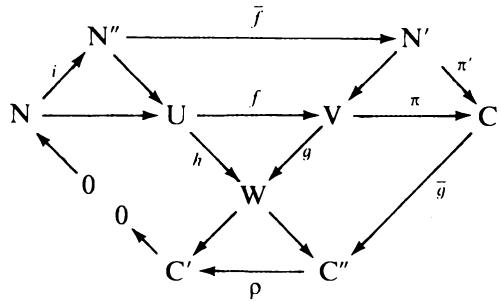
\includegraphics[keepaspectratio]{images/part002_9769358f.jpg}}\\
FIG. 1

By hypothesis N, N', C and C' are of finite dimension; hence the same is true of N'' and C''. By Cor. 2 (II, p.~295) we then have

\[
[ \mathrm{N}: \mathrm{L} ] - [ \mathrm{N} ^ {\prime \prime}: \mathrm{L} ] + [ \mathrm{N} ^ {\prime}: \mathrm{L} ] - [ \mathrm{C}: \mathrm{L} ] + [ \mathrm{C} ^ {\prime \prime}: \mathrm{L} ] - [ \mathrm{C} ^ {\prime}: \mathrm{L} ] = 0
\]

whence \(\chi(h) = \chi(f) + \chi(g)\) .

\subsection{Differential properties of finitely generated extensions}

THEOREM 4. --- Let P be a perfect field, L an extension of P and K a subextension of L; we suppose that L is a finitely generated extension of K. Then the canonical L-linear mapping \(\alpha: \Omega_{\mathrm{P}}(\mathrm{K}) \otimes_{\mathrm{K}} \mathrm{L} \to \Omega_{\mathrm{P}}(\mathrm{L})\) has index equal to the transcendence degree of L over K.

If E and F are two subextensions of L such that \(E \subset F\) , we denote by \(\alpha(F/E)\) the canonical F-linear mapping of \(\Omega_{\mathrm{P}}(\mathrm{E}) \otimes_{\mathrm{E}} F\) into \(\Omega_{\mathrm{P}}(\mathrm{F})\) and when it is defined, the index of \(\alpha(F/E)\) will be written \(d(F/E)\) . If E, F and G are three subextensions of L such that \(E \subset F \subset G\) , we have a commutative diagram

\[
\begin{array}{c} \Omega_ {\mathrm{P}} (\mathrm{F}) \otimes_ {\mathrm{F}} \mathrm{G} \xrightarrow {\alpha (\mathrm{G} / \mathrm{F})} \Omega_ {\mathrm{P}} (\mathrm{G}) \\ \alpha (\mathrm{F} / \mathrm{E}) \otimes_ {\mathrm{F}} \mathrm{Id} _ {\mathrm{G}} \Bigg | _ {\uparrow} \\ (\Omega_ {\mathrm{P}} (\mathrm{E}) \otimes_ {\mathrm{E}} \mathrm{F}) \otimes_ {\mathrm{F}} \mathrm{G} \xrightarrow {\beta} \Omega_ {\mathrm{P}} (\mathrm{E}) \otimes_ {\mathrm{E}} \mathrm{G} \end{array}
\]

where \(\beta\) is the canonical isomorphism defined in Prop. 2 (II, p.~278). Since the index is clearly invariant under extension by scalars and the index of an isomorphism is zero, Lemma 2 (V, p.~133) shows that the index \(d(\mathrm{G}/\mathrm{E})\) is defined when \(d(\mathrm{F}/\mathrm{E})\) and \(d(\mathrm{G}/\mathrm{F})\) are and then

\[
d (\mathrm{G} / \mathrm{E}) = d (\mathrm{G} / \mathrm{F}) + d (\mathrm{F} / \mathrm{E}).\tag{5}
\]

Since L is a finitely generated extension of K, Formula (5) and the Cor. of V, p.~111 shows that it is enough to consider the case where x exists such that \(L = K(x)\) ; further if x is algebraic over K, there exists a power q of the characteristic exponent of L such that \(x^{q}\) is separable algebraic over K (V, p.~44, Prop. 13). So it is enough to establish the equality \(d(\mathrm{L}/\mathrm{K}) = \operatorname{tr} \cdot \deg_{\mathrm{K}} \mathrm{L}\) in the three special cases below:

\begin{enumerate}
\def\labelenumi{\alph{enumi})}
\item
  \(x\) is transcendental over \(\mathbf{K}\) : then \(\alpha\) is injective and its cokernel is of rank 1 over \(\mathrm{L}(\mathrm{V},\mathrm{p}.129,\mathrm{Cor.})\) ; so we have \(d(\mathrm{L} / \mathrm{K}) = 1\) and also tr. \(\deg_{\mathbf{K}}\mathrm{L} = 1\) .
\item
  \(x\) is separable algebraic over \(\mathbf{K}\) : then \(\alpha\) is bijective (V, p.~130, Cor. 2), whence \(d(L / K) = 0\) ; clearly also tr. \(\deg_{\mathbf{K}}\mathbf{L} = 0\) .
\item
  The field L is of characteristic \(p \neq 0\) , \(x \notin K\) and \(x^{p} = a\) is in K: the cokernel C of \(\alpha\) is isomorphic to \(\Omega_{\mathrm{K}}(\mathrm{L})\) , and since \(\{x\}\) is a p-basis of L over K, the space C is of dimension 1 over L (V, p.~102, Th. 1). Since a is a p-th power in L, we have \(d_{L/P}a = 0\) and the kernel of \(\alpha\) contains the subspace R of \(U = \Omega_{\mathrm{P}}(\mathrm{K}) \otimes_{\mathrm{K}} L\) generated by \(d_{K/P}a \otimes 1\) . For each \(y \in K\) let \(\Delta(y)\) be the residue class of \(d_{K/P}y \otimes 1 \mod R\) ; then \(\Delta\) is a P-derivation of K into U/R such that \(\Delta(a) = 0\) . Prop. 5 (V, p.~101) shows that \(\Delta\) extends to a P-derivation D of L into U/R. Hence there exists an L-linear mapping \(\beta : \Omega_{\mathrm{P}}(\mathrm{L}) \to \mathrm{U}/\mathrm{R}\) such that \(D = \beta \circ d_{L/P}\) and \(\beta \circ \alpha\) is the canonical mapping of U onto U/R. This proves R to be the kernel of \(\alpha\) . Since P is perfect, we have \(P(K^{p}) = K^{p}\) , whence \(a \notin P(K^{p})\) and finally \(d_{K/P}a \neq 0\) (V, p.~103, Prop. 6). The kernel and cokernel of \(\alpha\) are thus of dimension 1, whence \(d(\mathrm{L}/\mathrm{K}) = 0\) , and we also have tr. deg \(_{K}L = 0\) .
\end{enumerate}

COROLLARY 1. --- Let L be a finitely generated extension of a field K of transcendence degree s. The vector space \(\Omega_{\mathrm{K}}(\mathrm{L})\) is of dimension \(\geqslant s\) over L, with equality if and only if L is separable over K.

Let P be the prime subfield of K. Let N be the kernel of \(\alpha\) , then by exactness of the sequence \((\mathrm{E}_{\mathrm{P},\mathrm{K},\mathrm{L}})(\mathrm{V},\mathrm{p}.128)\) and Th. 4, we have \([\Omega_{\mathrm{K}}(\mathrm{L}):\mathrm{L}] = s + [\mathrm{N}:\mathrm{L}]\) ; by V, p.~132, Cor., the extension L of K is separable if and only if N = 0. The corollary now follows.

COROLLARY 2. --- Let L be a finitely generated extension of a field K. For L to be algebraic and separable over K it is necessary and sufficient that \(\Omega_{\mathbf{K}}(\mathbf{L}) = 0\) .

This follows immediately from Cor. 1.

COROLLARY 3. --- Let K be a field of characteristic \(p \neq 0\) and L a finitely generated extension of K of transcendence degree s. If \([K:K^{p}]\) is finite, the same is true of \([L:L^{p}]\) and we have \([L:L^{p}] = p^{s} \cdot [K:K^{p}]\) .

Let P be the prime subfield of K. If \([K:K^{p}]\) is finite, then the vector space \(\Omega_{\mathrm{P}}(\mathrm{K})=\Omega_{\mathrm{K}^{\mathrm{p}}}\left(\mathrm{K}\right)\) is of finite dimension m over K, and we have \([K:K^{p}]=p^{m}(V,p.103,Th.2)\) ; the vector space \(\Omega_{\mathrm{P}}(\mathrm{K})\otimes_{\mathrm{K}}L\) is then of finite dimension m over L. Further, since K is of finite degree over \(K^{p}\) , the field \(\mathrm{K}(L^{p})\) is of finite degree over \(\mathrm{K}^{p}(L^{p})=L^{p}\) ; since the field L is a finitely generated extension of K and is algebraic over \(\mathrm{K}(L^{p})\) , it is an extension of finite degree of \(\mathrm{K}(L^{p})(\mathrm{V},p.18,Th.2)\) ; we thus conclude that L is of finite degree over \(L^{p}(V,p.10,Th.1)\) . Then \(\Omega_{\mathrm{P}}(\mathrm{L})\) is a vector space of finite dimension n over L and we have \([L:L^{p}]=p^{n}(V,p.103,Th.2)\) . By Lemma 1 (V, p.~132) the L-linear mapping \(\alpha:\Omega_{\mathrm{P}}(\mathrm{K})\otimes_{\mathrm{K}}L\to\Omega_{\mathrm{P}}(\mathrm{L})\) therefore has index n-m, whence n-m=s by Th. 4 (V, p.~133) and \(p^{n}=p^{s}\cdot p^{m}\) .

Remarks. --- 1) Let K be a field of characteristic \(p \neq 0\) and L an extension of K. We have \(\Omega_{\mathbf{K}}(\mathbf{L}) = 0\) if and only \(\mathbf{L} = \mathbf{K}(\mathbf{L}^p)\) (V, p.~103, Prop. 6). Therefore if L is finitely generated over K, then it is an algebraic and separable extension if and only if we have \(\mathbf{L} = \mathbf{K}(\mathbf{L}^p)\) . When L is not finitely generated over K, this result no longer holds generally as is shown by the case where L is the perfect closure of K.

\begin{enumerate}
\def\labelenumi{\arabic{enumi})}
\setcounter{enumi}{1}
\tightlist
\item
  Let K be a field, \(F_{1}, \ldots, F_{m}\) polynomials in \(K[X_{1}, \ldots, X_{n}]\) and L an extension of K generated by the elements \(x_{1}, \ldots, x_{n}\) . Suppose that the polynomials \(F_{1}, \ldots, F_{m}\) generate the ideal of \(K[X_{1}, \ldots, X_{n}]\) consisting of all polynomials F such that \(F(x_{1}, \ldots, x_{n}) = 0\) . From Prop. 1 (V, p.~127) and the universal property of the module of differentials (III, p.~569) we easily deduce the following result: the vector space \(\Omega_{K}(L)\) over L is generated by \(dx_{1}, \ldots, dx_{n}\) ; we have the relations
\end{enumerate}

\[
\sum_ {i = 1} ^ {n} \mathrm{D} _ {i} \mathrm{F} _ {j} (x _ {1}, \dots , x _ {n}) \cdot d x _ {i} = 0 \quad (\text { for } 1 \leqslant j \leqslant m);\tag{6}
\]

finally if \(u_1, \ldots, u_n\) are elements of \(L\) such that \(\sum_{i=1}^{n} u_i \cdot dx_i = 0\) , there exist elements \(v_1, \ldots, v_m\) of \(L\) such that \(u_i = \sum_{j=1}^{m} D_i F_j(x_1, \ldots, x_n) v_j\) for \(1 \leqslant i \leqslant n\) . Let us denote by \(r\) the rank of the matrix \((D_i F_j(x_1, \ldots, x_n))\) with \(n\) rows and \(m\) columns; let \(s\) be the transcendence degree of L over K. Then we have \([\Omega_{\mathrm{K}}(\mathrm{L}):\mathrm{L}]=n-r\) . Therefore the extension L of K is separable if and only if \(r+s=n\) (Cor. 1), and it is algebraic and separable if and only if r=n (Cor. 2).

\subsection{Separating transcendence bases}

DEFINITION 1. --- Let L be an extension of a field K. A transcendence basis B of L over K is said to be separating if the algebraic extension L of K(B) is separable.

If K has characteristic 0, every transcendence basis of L over K is separating because every algebraic extension of a field of characteristic 0 is separable (V, p.~37, Cor.). If an extension admits a separating transcendence basis, it is separable (V, p.~121, Prop. 6 and p.~122, Prop. 9). The following theorem shows that every finitely generated separable extension admits a separating transcendence basis; this restriction is essential (V, p.~177, Ex. 1).

THEOREM 5. --- Let K be a field, L an extension of K and \((x_{i})_{i\in I}\) a family of elements of L. If the family \((x_{i})_{i\in I}\) is a separating transcendence basis of L over K, then the family \((dx_{i})_{i\in I}\) is a basis of the vector space \(\Omega_{\mathrm{K}}(\mathrm{L})\) over L. The converse holds if L is a finitely generated separable extension of K.

Put \(\mathbf{M} = \mathbf{K}(x_i)_{i \in I}\) and denote by \(\alpha\) the canonical mapping of \(\Omega_{\mathbf{K}}(\mathbf{M}) \otimes_{\mathbf{M}} \mathbf{L}\) into \(\Omega_{\mathbf{K}}(\mathbf{L})\) . If \((x_i)_{i \in I}\) is a separating transcendence basis of L over K, the family \((d_{\mathbf{M}/\mathbf{K}} x_i)_{i \in I}\) is a basis of the vector M-space \(\Omega_{\mathbf{K}}(\mathbf{M})\) (V, p.~128, Prop. 3) and \(\alpha\) is an isomorphism of vector L-spaces since L is algebraic and separable over M (V, p.~130, Cor. 2). Since \(\alpha(d_{\mathbf{M}/\mathbf{K}} x_i \otimes 1) = d_{\mathbf{L}/\mathbf{K}} x_i\) , the family \((d_{\mathbf{L}/\mathbf{K}} x_i)_{i \in I}\) is thus a basis of \(\Omega_{\mathbf{K}}(\mathbf{L})\) over L.

Conversely, suppose that L is a separable finitely generated extension of K and that the family \((d_{L/K}x_{i})_{i\in I}\) is a basis of the vector space \(\Omega_{K}(L)\) over L. By Cor. 1 of V, p.~134, the transcendence degree of L over K is equal to the dimension of \(\Omega_{K}(L)\) over L, hence to the cardinal of I. From the exact sequence \((\mathrm{E}_{\mathrm{K},\mathrm{M},\mathrm{L}})(\mathrm{V},\mathrm{p}.128)\) we have \(\Omega_{\mathrm{M}}(\mathrm{L})=0\) ; since L is a finitely generated extension of M, Cor. 2 of V, p.~135 shows that L is algebraic and separable over \(\mathbf{M}=\mathbf{K}(x_{i})_{i\in I}\) ; since the transcendence degree of L over K is finite and equal to the cardinal of I, the family \((x_{i})_{i\in I}\) is a transcendence basis of L over K (V, p.~110, Cor. 1).

COROLLARY. --- Let L be a separable finitely generated extension of K and let S be a subset of L such that \(L = K(S)\) . Then there exists a separating transcendence basis B of L over K, contained in S.

Since \(\Omega_{\mathrm{K}}(\mathrm{L})\) is generated by the differentials of the elements of S, there exist s elements \(x_{1}, \ldots, x_{s}\) of S such that \((dx_{1}, \ldots, dx_{s})\) is a basis of \(\Omega_{\mathrm{K}}(\mathrm{L})\) over L. Now it suffices to apply Th. 5.

Remark. --- Let L be a separable finitely generated extension of a field K of characteristic \(p \neq 0\) ; there may exist transcendence bases of L which are not separating. It is enough to observe that \(\{X^{p}\}\) is a transcendence basis of \(\mathrm{K}(\mathbf{X})\) but \(\mathrm{K}(\mathbf{X})\) is a p-radical extension of degree p of \(\mathrm{K}(\mathbf{X}^{p})\) .

PROPOSITION 5. --- Let L and M be two extensions of a field K contained in a given extension and algebraically disjoint over K. If M is separable over K, then L(M) is separable over L.

It is enough to show that for every finite subset S of M, L(S) is separable over L (V, p.~122, Prop. 8). Let S be a finite subset of M. Since the field K(S) is separable over K, it has a separating transcendence basis B (Cor. of Th. 5). Since L and M are algebraically disjoint over K, B is a transcendence basis of L(B) over L (V, p.~113, Prop. 12). Further, every element of S is algebraic and separable over K(B), hence over L(B) (V, p.~39, Cor. 2). We deduce (V, p.~39, Prop. 6) that L(S) = L(B)(S) is algebraic and separable over L(B), hence L(S), is separable over L.

COROLLARY. --- If L and M are separable extensions, algebraically disjoint over K, then the field \(\mathbf{K}(\mathbf{L} \cup \mathbf{M})\) is separable over K.

For \(K(L \cup M) = L(M)\) is separable over L by Prop. 5 (because M is separable over K) and L is separable over K, whence the corollary (V, p.~122, Prop. 9).

\pandocbounded{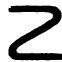
\includegraphics[keepaspectratio]{images/part002_2c83366d.jpg}}

The hypothesis that the extensions L and M are algebraically disjoint is indispensable in Prop. 5 and its corollary. For let K be an imperfect field of characteristic \(p \neq 0\) and E an extension of the form \(\mathrm{K}(x, a)\) with x transcendental over K and a p-radical of height 1 over K; put \(\mathrm{L} = \mathrm{K}(x)\) and \(\mathrm{M} = \mathrm{K}(x + a)\) . Then \(x + a\) is transcendental over K (if not, \(x = (x + a) - a\) would be algebraic over K) and the fields L and M are separable over K. However, \(\mathrm{K}(\mathrm{L} \cup \mathrm{M}) = \mathrm{K}(x, a)\) is p-radical of degree p over \(\mathrm{L} = \mathrm{K}(x)\) and is not separable over L, nor over K.

\section{REGULAR EXTENSIONS}

\subsection{Complements on the relative separable algebraic closure}

THEOREM 1 (Zariski). --- Let K be a field, L an extension of K, \(K_{1}\) the relative separable algebraic closure of K in L (V, p.~44), \(K_{2}\) the relative algebraic closure of K in L (V, p.~19) and \((\mathbf{X}_{i})_{i\in I}\) a family of indeterminates. Then \(\mathrm{K}_{1}(\mathbf{X}_{i})_{i\in I}\) is the relative separable algebraic closure of \(\mathrm{K}(\mathbf{X}_{i})_{i\in I}\) in \(\mathrm{L}(\mathbf{X}_{i})_{i\in I}\) and \(\mathrm{K}_{2}(\mathbf{X}_{i})_{i\in I}\) is the relative algebraic closure of \(\mathrm{K}(\mathbf{X}_{i})_{i\in I}\) in \(\mathrm{L}(\mathbf{X}_{i})_{i\in I}\) .

\begin{enumerate}
\def\labelenumi{\Alph{enumi})}
\tightlist
\item
  Suppose that E is a field and F an extension field of E and that every element of F which is separable algebraic over E belongs to E. Let u be an element of \(F(X)\) which is separable algebraic over \(E(X)\) ; we shall show that u belongs to \(E(X)\) . There exist in \(F(X)\) two relatively prime polynomials P and Q such that u = P/Q and we may take Q to be monic. Let S be the finite subset of F consisting of the coefficients of P and Q, \(F_{0} = E(S)\) and let \(\Delta\) be an E-derivation of \(\mathbf{F}_0\) into \(\mathbf{F}_0\) . Let \(D\) be the derivation of \(\mathrm{F}_0(\mathbf{X})\) into itself which agrees with \(\Delta\) on \(\mathbf{F}_0\) and maps \(X\) to 0 (V, p.~128, Prop. 3).
\end{enumerate}

Since \(u \in F_0(X)\) is separable algebraic over \(E(X)\) and \(D\) is zero on \(E(X)\) , we have \(D(u) = 0\) (V, p.~129, Prop. 4), whence \(D(P).Q = P.D(Q)\) . Since \(P\) and \(Q\) are relatively prime, we conclude that \(Q\) divides \(D(Q)\) (IV, p.~13, Cor. 4). Now \(Q\) may be written in the form

\[
\mathrm{Q} (\mathrm{X}) = \mathrm{X} ^ {n} + a _ {1} \mathrm{X} ^ {n - 1} + \dots + a _ {n - 1} \mathrm{X} + a _ {n}
\]

with \(a_1, \ldots, a_n\) in \(\mathbf{F}_0\) ; since \(\mathbf{D}(x) = 0\) , we thus have

\[
\mathrm{D} (\mathrm{Q}) = \Delta (a _ {1}) \mathrm{X} ^ {n - 1} + \dots + \Delta (a _ {n - 1}) \mathrm{X} + \Delta (a _ {n})\tag{1}
\]

whence \(\deg D(Q) < \deg Q\) . Since \(Q\) divides \(D(Q)\) , this is possible only if \(D(Q) = 0\) . But then \(D(P) = 0\) because \(D(P) \cdot Q = P \cdot D(Q)\) . Now (1) and a similar formula for \(P\) show that \(\Delta\) annihilates the set \(S\) of coefficients of \(P\) and \(Q\) , whence \(\Delta = 0\) , because \(F_0 = E(S)\) . By \(V\) , p.~135, Cor. 2, the finitely generated extension \(F_0\) of \(E\) is thus separable algebraic; by the hypotheses on \(E\) and \(F\) we have \(F_0 = E\) , so finally \(u \in E(X)\) .

\begin{enumerate}
\def\labelenumi{\Alph{enumi})}
\setcounter{enumi}{1}
\item
  Suppose now that E is relatively algebraically closed in the extension field F and denote by p the characteristic exponent of E. Let u be an element of \(F(X)\) which is algebraic over \(E(X)\) . There exists an integer \(f \geqslant 0\) such that \(v = u^{p^f}\) is separable algebraic over \(E(X)\) (V, p.~44, Prop. 13). By A) we thus have \(v \in E(X)\) . There exists a unique representation of u in the form P/Q with relatively prime polynomials P and Q in F{[}X{]} and Q monic; we have a similar decomposition \(v = P_1 / Q_1\) with \(P_1\) and \(Q_1\) relatively prime in E{[}X{]} and \(Q_1\) monic. It follows that \(P_1 / Q_1 = P^{p^f} / Q^{p^f}\) ; the polynomials \(P^{p^f}\) and \(Q^{p^f}\) are relatively prime in F{[}X{]} (IV, p.~13, Cor. 6), like \(P_1\) and \(Q_1\) , and \(Q^{p^f}\) is monic. It follows that \(P^{p^f} = P_1 \in E[X]\) and \(Q^{p^f} = Q_1 \in E[X]\) . Therefore the coefficients of P and Q are p-radical over E, and hence belong to E because E is relatively algebraically closed in F. We thus have \(P \in E[X]\) , \(Q \in E[X]\) and finally \(u \in E(X)\) . This proves \(E(X)\) to be relatively algebraically closed in F(X).
\item
  We use the notation of Theorem 1. Since \(\mathbf{K}_1\) is a separable algebraic extension of \(\mathbf{K}\) , the extension \(\mathbf{K}_1(\mathbf{X}_i)_{i\in I}\) of \(\mathbf{K}(\mathbf{X}_i)_{i\in I}\) is algebraic and separable (V, p.~39, Prop. 6). Moreover, every element of \(L\) which is algebraic and separable over \(\mathbf{K}_1\) belongs to \(\mathbf{K}_1\) (V, p.~44, Prop. 13, a)). Let \(J\) be a finite subset of \(I\) ; by an immediate induction on the cardinal of \(J\) we deduce from \(A\) ) that every element of \(\mathrm{L}(\mathbf{X}_i)_{i\in J}\) which is algebraic and separable over \(\mathbf{K}(\mathbf{X}_i)_{i\in J}\) belongs to \(\mathbf{K}_1(\mathbf{X}_i)_{i\in J}\) . Finally let \(u\) be an element of \(\mathrm{L}(\mathbf{X}_i)_{i\in I}\) algebraic and separable over \(\mathbf{K}(\mathbf{X}_i)_{i\in I}\) ; there exists a finite subset \(J\) of \(I\) such that \(u\) belongs to \(\mathrm{L}(\mathbf{X}_i)_{i\in J}\) and is algebraic and separable over \(\mathbf{K}(\mathbf{X}_i)_{i\in J}\) ; by what has been said, \(u\) belongs to \(\mathbf{K}_1(\mathbf{X}_i)_{i\in J}\) and a fortiori to \(\mathbf{K}_1(\mathbf{X}_i)_{i\in I}\) .
\end{enumerate}

We have thus deduced from \(A\) that \(\mathrm{K}_1(\mathbf{X}_i)_{i\in I}\) is the relative separable closure of \(\mathrm{K}(\mathbf{X}_i)_{i\in I}\) in \(\mathrm{L}(\mathbf{X}_i)_{i\in I}\) ; in the same way it follows from \(B\) that \(\mathrm{K}_2(\mathbf{X}_i)_{i\in I}\) is the relative algebraic closure of \(\mathrm{K}(\mathbf{X}_i)_{i\in I}\) in \(\mathrm{L}(\mathbf{X}_i)_{i\in I}\) .

\subsection{The tensor product of extensions}

PROPOSITION 1. --- Let \(\Omega\) be an extension of a field \(K\) and let \(L, M\) be two subextensions of \(\Omega\) which are algebraically disjoint over \(K\) . Suppose that the relative separable algebraic closure of \(K\) in \(L\) is equal to \(K^1\) . Let \(\varphi\) be the K-algebra homomorphism of \(L \otimes_K M\) into \(\Omega\) mapping \(x \otimes y\) to \(xy\) for \(x \in L\) , \(y \in M\) , and let \(\mathfrak{p}\) be the kernel of \(\varphi\) . Then \(\mathfrak{p}\) is the set of nilpotent elements of \(L \otimes_K M\) and this is the smallest prime ideal of \(L \otimes_K M\) .

On replacing \(\Omega\) by an algebraic closure if necessary, we may suppose \(\Omega\) algebraically closed. Let B be a transcendence basis of M over K, N the relative algebraic closure of \(\mathrm{K}(\mathrm{B})\) in \(\Omega\) and \(\mathrm{N}_{s}\) (resp. \(N_{r}\) ) the set of elements of N which are separable (resp. p-radical) over \(\mathrm{K}(\mathrm{B})\) . We remark that M is algebraic over \(\mathrm{K}(\mathrm{B})\) , so that N is the relative algebraic closure of M in \(\Omega\) .

\pandocbounded{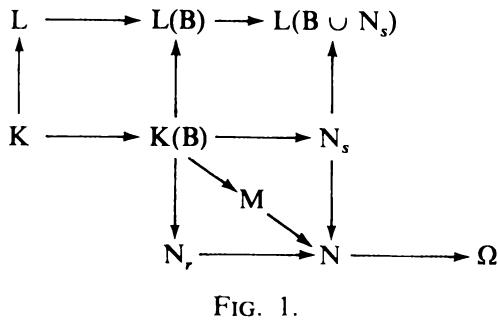
\includegraphics[keepaspectratio]{images/part002_5eeda79f.jpg}}

Let us define the following chain of homomorphisms :

\[
\begin{array}{r l} & {\mathrm{L} \otimes_ {\mathrm{K}} \mathrm{M} \xrightarrow {\alpha} \mathrm{L} \otimes_ {\mathrm{K}} \mathrm{N} \xrightarrow {\beta} (\mathrm{L} \otimes_ {\mathrm{K}} \mathrm{K} (\mathrm{B})) \otimes_ {\mathrm{K} (\mathrm{B})} \mathrm{N} \xrightarrow {\gamma} \mathrm{L} (\mathrm{B}) \otimes_ {\mathrm{K} (\mathrm{B})} \mathrm{N}} \\ & {\xrightarrow {\delta} \mathrm{L} (\mathrm{B}) \otimes_ {\mathrm{K} (\mathrm{B})} \mathrm{N}_s \otimes_ {\mathrm{K} (\mathrm{B})} \mathrm{N}_r \xrightarrow {\varepsilon} \mathrm{L} (\mathrm{B} \cup \mathrm{N}_s) \otimes_ {\mathrm{K} (\mathrm{B})} \mathrm{N}_r \xrightarrow {\zeta} \Omega .} \end{array}
\]

We have \(\alpha = \mathrm{Id}_{\mathbf{L}} \otimes u\) where \(u\) is the canonical injection of M into N, hence \(\alpha\) is injective. The mapping \(\beta\) is the isomorphism of commutative groups which maps \(x \otimes y\) to \((x \otimes 1) \otimes y\) (II, p.~278, Prop. 2) for \(x \in L\) and \(y \in N\) . We have \(\gamma = v \otimes \mathrm{Id}_{\mathbf{N}}\) , where \(v\) is the K-algebra homomorphism of \(\mathrm{L} \otimes_{\mathbf{K}} \mathrm{K}(\mathrm{B})\) into \(\mathrm{L}(\mathrm{B})\) which maps \(x \otimes y\) to \(xy\) , for \(x \in L\) and \(y \in \mathrm{K}(\mathrm{B})\) ; since L and M are algebraically disjoint over K, Prop. 14 (V, p.~114) shows that L and K(B) are linearly disjoint over K, in other words, \(v\) is injective, hence \(\gamma\) is injective. Since N is a quasi-Galois extension of K(B), there exists (V, p.~76, Prop. 13) a K(B)-algebra isomorphism \(w\) of \(\mathrm{N}_s \otimes_{\mathrm{K}(\mathrm{B})} \mathrm{N}_r\) onto N mapping \(x \otimes y\) to \(xy\) for \(x \in \mathbf{N}_s\) and \(y \in \mathbf{N}_r\) ; we denote by \(\delta\) the isomorphism \(\mathrm{Id}_{\mathrm{L(B)}} \otimes w^{-1}\) . By Th. 1 (V, p.~137) and the hypothesis on the extension L of K, every element of L(B) which is algebraic and separable over K(B) belongs to K(B); in particular, we have L(B) \(\cap\) N \(_s\) = K(B). Since N \(_s\) is a Galois extension of K(B), Th. 5 (V, p.~71) shows that there exists a K(B)-algebra isomorphism \(w'\) of L(B) \(\otimes_{\mathrm{K(B)}} \mathrm{N}_s\) onto L(B \(\cup\) N \(_s\) ) mapping \(x \otimes y\) to \(xy\) for \(x \in L(B)\) and \(y \in \mathrm{N}_s\) ; we denote by \(\varepsilon\) the isomorphism \(w' \otimes \mathrm{Id}_{\mathrm{N}_r}\) . Finally, \(\zeta\) is the K-algebra homomorphism mapping \(x \otimes y\) to \(xy\) for \(x \in L(B \cup \mathrm{N}_s)\) and \(y \in \mathrm{N}_r\) .

What has been said shows that \(\eta = \varepsilon \delta \gamma \beta \alpha\) is an injective K-algebra homomorphism of \(L \otimes_{K} M\) into \(L(B \cup N_s) \otimes_{K(B)} N_r\) . Further, every element of \(M\) is of the form \(\sum_{i=1}^{n} a_i b_i\) with \(a_i \in N_s\) and \(b_i \in N_r\) for \(1 \leqslant i \leqslant n\) ; hence we obtain \(\varphi = \zeta \eta\) .

The kernel \(\mathfrak{p}\) of \(\varphi\) is a prime ideal of \(\mathbf{L} \otimes_{\mathbb{K}} \mathbf{M}\) , hence every nilpotent element of \(\mathbf{L} \otimes_{\mathbb{K}} \mathbf{M}\) belongs to \(\mathfrak{p}\) , by Prop. 2 (V, p.~118). Conversely let \(a\) be an element of \(\mathfrak{p}\) ; put \(\eta(a) = \sum_{i=1}^{s} b_i \otimes c_i\) with \(b_i \in \mathbf{L}(\mathbf{B} \cup \mathbf{N}_s)\) and \(c_i \in \mathbf{N}_r\) for \(1 \leqslant i \leqslant s\) . Since

\(N_{r}\) is a p-radical extension of \(K(B)\) , there exists an integer \(f \geqslant 0\) such that \(c_{i}^{p^{f}}\) belongs to \(K(B)\) for \(1 \leqslant i \leqslant s\) (where p is the characteristic exponent of K). But we have

\[
\eta \left(a ^ {p ^ {f}}\right) = \sum_ {i = 1} ^ {s} b _ {i} ^ {p ^ {f}} \otimes c _ {i} ^ {p ^ {f}} = \left(\sum_ {i = 1} ^ {s} b _ {i} ^ {p ^ {f}} c _ {i} ^ {p ^ {f}}\right) \otimes 1 = \zeta \eta (a) ^ {p ^ {f}} \otimes 1 = 0
\]

and since \(\eta\) is injective we finally have \(a^{p^{f}} = 0\) . We have thus shown \(\mathfrak{p}\) to be the set of all nilpotent elements of \(\mathrm{L} \otimes_{\mathrm{K}} \mathrm{M}\) . Now every prime ideal of \(\mathrm{L} \otimes_{\mathrm{K}} \mathrm{M}\) contains \(\mathfrak{p}\) by Prop. 2 (V, p.~118).

COROLLARY. --- Let L and M be two extensions of a field K. Suppose that the relative separable algebraic closure of K in L is equal to K. Then the set p of nilpotent elements of \(L \otimes_{K} M\) is a prime ideal. If moreover L or M is separable over K, then \(L \otimes_{K} M\) is an integral domain.

We may assume that L and M are algebraically disjoint subextensions of an extension \(\Omega\) of K (V, p.~116, Th. 5); then p is a prime ideal by Prop. 1 (V, p.~139). If moreover L or M is separable over K, then \(L \otimes_{K} M\) is a reduced ring by the definition of separable extension (V, p.~119, Def. 1); so p = 0 and \(L \otimes_{K} M\) is an integral domain because p was prime.

\subsection{Regular algebras}

DEFINITION 1. --- Let K be a field. An algebra A over K is said to be regular if L ⊗K A is an integral domain for every extension L of K.

A regular algebra is in particular an integral domain, hence commutative.

PROPOSITION 2. --- Let A and B be two algebras over a field K. If A is an integral domain and B is regular then \(A \otimes_{K} B\) is an integral domain.

Let \(L\) be the field of fractions of \(A\) . Since \(B\) is a regular \(K\) -algebra, \(L \otimes_K B\) is an integral domain, hence so is \(A \otimes_K B\) , since it is isomorphic to a subring of \(L \otimes_K B\) .

PROPOSITION 3. --- Let K be a field.

\begin{enumerate}
\def\labelenumi{\alph{enumi})}
\item
  Every subalgebra of a regular K-algebra is itself regular.
\item
  The tensor product of two regular K-algebras is again regular.
\item
  Let A be a K-algebra and \(K'\) an extension of K. For A to be regular it is necessary and sufficient that the \(K'\) -algebra \(\mathrm{A}_{(\mathbb{K}')}\) derived from A by extension of scalars should be regular.
\end{enumerate}

The proof of \(a\) (resp. \(c\) ) is identical to that of part \(a\) (resp. \(d\) ) of Prop. 3, V, p.~119, after replacing everywhere « reduced ring » by « integral domain » and « separable algebra » by « regular algebra ». Let us prove \(b\) ).

Let A and B be two regular K-algebras. Let L be an extension of K. Since A is regular, the ring \(L \otimes_{K} A\) is an integral domain. By Prop. 2, the ring \((L \otimes_{K} A) \otimes_{K} B\) is an integral domain, because B is regular. Finally, the ring \(L \otimes_{K} (A \otimes_{K} B)\) is isomorphic to \((L \otimes_{K} A) \otimes_{K} B\) , and hence is an integral domain. This shows \(A \otimes_{K} B\) to be a regular K-algebra.

\subsection{Regular extensions}

DEFINITION 2. --- An extension of a field K is said to be regular if it is regular as K-algebra.

PROPOSITION 4. --- Let A be an algebra over field K which is an integral domain, and E its field of fractions. Let L be an extension of K; if the ring \(L \otimes_{K} A\) is an integral domain the same is true of \(L \otimes_{K} E\) .

If \(L \otimes_{K} A\) is an integral domain, it may be embedded in its field of fractions F. Write \(u(x) = x \otimes 1\) for \(x \in L\) and denote by v the K-homomorphism of E into F which extends the injective homomorphism \(y \mapsto 1 \otimes y\) of A into F. By Prop. 6 (V, p.~14) the subfields \(u(L)\) and \(v(E)\) of F are linearly disjoint over K; therefore the homomorphism \(u * v\) of \(L \otimes_{K} E\) into F (V, p.~12) is injective. This shows \(L \otimes_{K} E\) to be an integral domain.

COROLLARY. --- For A to be a regular K-algebra it is necessary and sufficient that its field of fractions should be a regular extension of K.

The condition is necessary by Prop. 4 and sufficient by Prop. 3, a).

PROPOSITION 5. --- Every pure extension of a field K is regular.

By the preceding corollary it is enough to prove that every polynomial algebra \(A = K[X_{i}]_{i \in I}\) is a regular K-algebra. Let L be an extension of \(K\) ; the ring \(L \otimes_{K} A\) is isomorphic to \(L[X_{i}]_{i \in I}\) (III, p.~449, Remark 2), and hence an integral domain (IV, p.~9, Prop. 8).

PROPOSITION 6. --- Let L be an extension of a field K. If L is regular, then every subextension of L is regular. Conversely, if every finitely generated subextension of L is regular, then L is regular.

The first assertion follows from Prop. 3, a).

Let M be an extension of K and let U be the set of all finitely generated subextensions of L. For each \(E \in U\) , the ring \(M \otimes_{K} E\) may be identified with a subring of \(M \otimes_{K} L\) and we thus have an increasing directed family of subrings of \(M \otimes_{K} L\) whose union is \(M \otimes_{K} L\) . Now the second assertion follows immediately.

PROPOSITION 7. --- Let L be an extension of a field K and M an L-algebra (for example, an extension of L). If L is regular over K and M is a regular L-algebra, then M is regular as K-algebra.

Let E be an extension of K; since L is regular over K, \(E \otimes_{K} L\) is an integral domain. By Prop. 2 (V, p.~141) the ring \((\mathrm{E} \otimes_{\mathrm{K}} \mathrm{L}) \otimes_{\mathrm{L}} \mathrm{M}\) is thus an integral domain and the same is true of the ring \(E \otimes_{K} M\) isomorphic to it (II, p.~278, Prop. 2). Hence the result.

PROPOSITION 8. --- Let L and M be two extensions of a field K.

\begin{enumerate}
\def\labelenumi{\alph{enumi})}
\item
  If \(\mathbf{M}\) is regular over \(\mathbf{K}\) , then the field of fractions of the integral domain \(\mathbf{L} \otimes_{\mathbf{K}} \mathbf{M}\) is a regular extension of \(\mathbf{L}\) .
\item
  If L and M are regular extensions of K, the same is true of the field of fractions of L ⊗\_K M.
\end{enumerate}

Assertion a) follows from Prop. 3, c) (V, p.~141) and the Cor. of V, p.~141; Assertion b) follows from Prop. 3, b) (V, p.~141) and the Cor. of V, p.~141.

\subsection{Characterization of regular extensions}

PROPOSITION 9. --- Let K be a field, \(\bar{K}\) an algebraic closure of K and L an extension of K. Then the following conditions are equivalent:

\begin{enumerate}
\def\labelenumi{\alph{enumi})}
\item
  L is separable over K and K is relatively algebraically closed in L.
\item
  L is a regular extension of K.
\item
  The ring \(\bar{\mathbf{K}}\otimes_{\mathbb{K}}\mathbf{L}\) is an integral domain.
\item
  Let \(\bar{L}\) be an algebraic closure of L. Then L is linearly disjoint over K from the relative algebraic closure of K in \(\bar{L}\) .
\end{enumerate}

Moreover, when these conditions hold, then \(\bar{\mathbf{K}}\otimes_{\mathbf{K}}\mathbf{L}\) is a field.

\(a) \Rightarrow b)\) : Let M be an extension of K. Under the hypotheses of \(a\) ), the ring M \(\otimes_{K} L\) is an integral domain, by V, p.~140, Cor.

\(b) \Rightarrow c)\) : This follows from Def. 2.

\(c) \Rightarrow d): \text{With the notation of } d) \text{ we can identify } \bar{\mathbf{K}} \text{ with the relative algebraic closure of } \mathbf{K} \text{ in } \bar{\mathbf{L}} (\mathbf{V}, \text{ p. 22, Ex. 2}). \text{ Suppose that the ring } \mathbf{A} = \bar{\mathbf{K}} \otimes_{\mathbf{K}} \mathbf{L} \text{ is an integral domain. Let } \mathbf{E} \text{ be a subextension of } \bar{\mathbf{K}} \text{ of finite degree over } \mathbf{K}; \text{ the subring}\)

\(E \otimes_{K} L\) of A is an integral domain and hence is an algebra of finite degree over L; by the Cor. of V, p.~10 it is a field. Since \(\bar{K}\) is the union the increasing directed set of extensions E of the above type, A is a field (V, p.~11, Prop. 3). The canonical homomorphism of A into \(\bar{L}\) mapping \(x \otimes y\) to xy (for \(x \in \bar{K}\) and \(y \in L\) ) is therefore injective, so L and \(\bar{K}\) are linearly disjoint over K.

\(d) \Rightarrow a): \text{Under the hypotheses of } d) \text{ we have } L \cap \bar{K} = K, \text{ so } K \text{ is relatively algebraically closed in } L; \text{ further if } p \text{ is the characteristic exponent of } K, \text{ the field } L \text{ is linearly disjoint from } K^{p^{-\infty}} \text{ over } K, \text{ hence } L \text{ is separable over } K (V, p. 123, Cor. 1).\)

COROLLARY 1. --- Let A be an algebra over a field K. For A to be a regular K-algebra it is necessary and sufficient for the ring \(\bar{\mathbf{K}}\otimes_{\mathbf{K}}\mathbf{A}\) to be an integral domain.

The stated condition is clearly necessary. Conversely, assume that \(\bar{K} \otimes_{K} A\) is an integral domain and denote by E the field of fractions of A. By Prop. 4 (V, p.~141) the ring \(\bar{K} \otimes_{K} E\) is an integral domain, hence E is a regular extension of K, by Prop. 9; by V, p.~141, Cor., we conclude that A is regular as K-algebra.

COROLLARY 2. --- Let K be an algebraically closed field. Every K-algebra which is an integral domain is a regular K-algebra. In particular, every extension of K is regular.

This follows from Cor. 1.

COROLLARY 3. --- Let K be an algebraically closed field. If A and B are two K-algebras which are integral domains, then the same is true of A ⊗\_K B.

By Cor. 2, A and B are regular K-algebras, and it suffices to apply Prop. 2 (V, p.~141).

\subsection{Application to composite extensions}

PROPOSITION 10. -- Let L and M be two extensions of a field K and (E, u, v) a composite extension of L and M (V, p.~12). Suppose that the ring L ⊗\_K M is an integral domain and that the subextensions u(L) and v(M) of E are algebraically disjoint over K. Then u(L) and v(M) are linearly disjoint over K.

Put \(w = u * v\) (V, p.~12), denote by F the field of fractions of the integral domain \(L \otimes_{K} M\) and identify L (resp. M) with a subfield of F by means of the mapping \(x \mapsto x \otimes 1\) (resp. \(y \mapsto 1 \otimes y\) ); then the restriction of w to L (resp. M) is u (resp. v). Let B be a transcendence basis of M over K (V, p.~109, Th. 1).

By hypothesis \(u(\mathbf{L})\) and \(v(\mathbf{M})\) are algebraically disjoint over \(\mathbf{K}\) ; therefore (V, p.~114, Prop. 14), \(u(\mathbf{L})\) and \(v(\mathbf{K}(\mathbf{B}))\) are linearly disjoint over \(\mathbf{K}\) . Thus there exists a K-homomorphism \(u': \mathbf{L}(\mathbf{B}) \to \mathbf{E}\) which agrees with \(u\) on \(\mathbf{L}\) and with \(v\) ou \(\mathbf{K}(\mathbf{B})\) . By construction \(\mathbf{L}\) and \(\mathbf{M}\) are linearly disjoint over \(\mathbf{K}\) in \(\mathbf{F}\) ; by Prop. 8 (V, p.~15) the subfields \(\mathbf{L}(\mathbf{B})\) and \(\mathbf{M}\) of \(\mathbf{F}\) are linearly disjoint over \(\mathbf{K}(\mathbf{B})\) . It follows that there exists a K-homomorphism \(w' \colon \mathbf{M}[\mathrm{L}(\mathrm{B})] \to \mathrm{E}\) which agrees with \(u'\) on \(\mathrm{L}(\mathrm{B})\) and with \(v\) on \(\mathbf{M}\) . But the field \(F\) is generated by \(\mathbf{M} \cup \mathrm{L}(\mathrm{B})\) and \(\mathbf{M}\) is algebraic over \(\mathbf{K}(\mathbf{B})\) ; we thus have \(\mathbf{M}[\mathrm{L}(\mathbf{B})] = F(\mathbf{V}, p. 18, Cor. 2)\) . Hence we conclude that \(w'\) is a K-isomorphism of \(F\) onto \(E\) whose restriction to \(L\) (resp. \(M\) ) is \(u\) (resp. \(v\) ). This shows \(u(L)\) and \(v(M)\) to be linearly disjoint over \(K\) .

COROLLARY 1. --- Let \(\Omega\) be an extension of a field \(K\) and \(L\) a subextension of \(\Omega\) which is regular over \(K\) . Every subextension \(M\) of \(\Omega\) which is algebraically disjoint from \(L\) over \(K\) is linearly disjoint.

The ring \(L \otimes_{K} M\) is an integral domain by definition of regular extension and it suffices now to apply Prop. 10.

COROLLARY 2. --- Let \(\Omega\) be an extension of a field \(K\) and \(L\) , \(M\) two subextensions of \(\Omega\) . Suppose that \(L\) is separable over \(K\) and that the relative separable closure of \(K\) in \(M\) is equal to \(K\) . If \(L\) and \(M\) are algebraically disjoint over \(K\) , then they are linearly disjoint over \(K\) .

By Prop. 10 it is enough to remark that the ring \(\mathbf{L} \otimes_{\mathbf{K}} \mathbf{M}\) is an integral domain (V, p.~140, Cor.).

\BourbakiExercises

\BourbakiExerciseGroup

\begin{enumerate}
\def\labelenumi{\arabic{enumi})}
\item
  Let A be a not necessarily commutative ring, not zero and without divisors of zero (I, p.~98). Show that if there exists an integer \(m \geqslant 1\) such that \(m\mathbf{A} = 0\) , then the set of all integers having this property is an ideal \(p\mathbf{Z}\) , where \(p\) is a prime number, and A is a ring of characteristic \(p\) .
\item
  Let \(m, n\) be integers such that \(0 \leqslant n \leqslant m\) . Let \(p\) be a prime number and let \(m = \alpha_0 + \alpha_1p + \cdots + \alpha_rp^r\) and \(n = \beta_0 + \beta_1p + \cdots + \beta_rp^r\) be the expansions of \(m\) and \(n\) in base \(p\) , where we thus have \(0 \leqslant \alpha_i < p\) , \(0 \leqslant \beta_i < p\) for \(0 \leqslant i \leqslant r\) ; suppose that \(\alpha_r \neq 0\) . Show that \(\binom{m}{n} \equiv 0 (\bmod p)\) if \(\beta_i > \alpha_i\) for at least one index \(i\) . If on the other hand, \(\beta_i \leqslant \alpha_i\) for \(0 \leqslant i \leqslant r\) , then
\end{enumerate}

\[
\binom {m} {n} \equiv \binom {\alpha_ {0}} {\beta_ {0}} \dots \binom {\alpha_ {r}} {\beta_ {r}} \pmod {p}  .
\]

(In \((\mathbf{Z} / p\mathbf{Z})[\mathbf{X}]\) we have \((1 + \mathbf{X})^m = (1 + \mathbf{X})^{\alpha_0}(1 + \mathbf{X}^p)^{\alpha_1}\dots (1 + \mathbf{X}^{p^r})^{\alpha_r})\)

\begin{enumerate}
\def\labelenumi{\arabic{enumi})}
\setcounter{enumi}{2}
\tightlist
\item
  Let \(\mathbf{A}\) be a commutative ring. For every polynomial \(f \in \mathbf{A}[\mathbf{X}]\) we write in the polynomial ring \(\mathbf{A}[\mathbf{X}, \mathbf{Y}]\) of polynomials in two indeterminates over \(\mathbf{A}\) ,
\end{enumerate}

\[
f (\mathbf {X} + \mathbf {Y}) = \sum_ {m = 0} ^ {\infty} \Delta_ {m} f (\mathbf {X}) \mathbf {Y} ^ {m},
\]

where \(\Delta_{m}\) is thus an A-linear mapping of A{[}X{]} into itself.\\
a) If Z is an indeterminate and \(\tau_{Z}\) the A-linear mapping of A{[}X{]} into A{[}X, Z{]} such that \(\tau_{Z}f = f(X + Z)\) , show that \(\tau_{Z} \circ \Delta_{m} = \Delta_{m} \circ \tau_{Z}\) (where on the right \(\Delta_{m}\) is the mapping defined above in the ring B{[}X{]}, where B = A{[}Z{]}). Deduce that in A{[}X{]} we have

\[
\Delta_ {m} \Delta_ {n} = \Delta_ {n} \Delta_ {m} = \binom {m + n} {m} \Delta_ {m + n}
\]

for integers \(m, n \geqslant 0\) (cf.~IV, p.~8).

\begin{enumerate}
\def\labelenumi{\alph{enumi})}
\setcounter{enumi}{1}
\tightlist
\item
  Suppose that A is a ring of characteristic p \textgreater{} 0 and for each integer \(k \geqslant 0\) put \(D_{k} = \Delta_{p^{k}}\) . Show that if \(f \in A[X]\) and \(g \in A[X^{p^{k}}]\) then \(D_{k}(fg) = g \cdot D_{k}f + f \cdot D_{k}g\) .
\end{enumerate}

Every polynomial \(f \in \mathbf{A}[\mathbf{X}]\) can be uniquely written in the form \(f(\mathbf{X}) = \sum_{m=0}^{\infty} \mathbf{X}^{mp^k} g_m(\mathbf{X})\) where \(\deg(g_m) < p^k\) ; show that

\[
\mathrm{D} _ {k} f (\mathbf {X}) = \sum_ {m = 0} ^ {\infty} m \mathbf {X} ^ {(m - 1) p ^ {k}} g _ {m} (\mathbf {X})
\]

and deduce that \(D_{k}^{p}=0\) .

\begin{enumerate}
\def\labelenumi{\alph{enumi})}
\setcounter{enumi}{2}
\tightlist
\item
  For every integer m \textgreater{} 0 let \(m = \alpha_{0} + \alpha_{1}p + \cdots + \alpha_{k}p^{k}\) be the expansion of m in base p (Set Theory, III, p.~177), where thus \(0 \leqslant \alpha_{j} < p\) for \(0 \leqslant j \leqslant k\) ; suppose that \(\alpha_{k} \neq 0\) . Show that
\end{enumerate}

\[
\Delta_ {m} = \left(\frac {1}{\alpha_ {0} !} D _ {0} ^ {\alpha_ {0}}\right) \left(\frac {1}{\alpha_ {1} !} D _ {1} ^ {\alpha_ {1}}\right) \dots \left(\frac {1}{\alpha_ {k} !} D _ {k} ^ {\alpha_ {k}}\right).
\]

(If \(\Delta_m'\) is the right-hand side of this relation, note that if we introduce the expansion \(f(\mathbf{X} + \mathbf{Y}) = \sum_{q=0}^{\infty} f_q(\mathbf{Y}) \mathbf{X}^q\) , we have \(\Delta_m' f(\mathbf{X} + \mathbf{Y}) = \sum_{q=0}^{\infty} f_q(\mathbf{Y}) \Delta_m'(\mathbf{X}^q)\) and deduce that this may be written \(\Delta_m' f(\mathbf{X} + \mathbf{Y}) = f_m(\mathbf{X}) + \mathbf{Y} g(\mathbf{X}, \mathbf{Y})\) , where \(g\) is a polynomial.)

\begin{enumerate}
\def\labelenumi{\arabic{enumi})}
\setcounter{enumi}{3}
\tightlist
\item
  Let \(\mathbf{G}\) be a commutative group, written additively, and let \(p\) be a prime number. Denote by \(\mathbf{G}\left[\frac{1}{p}\right]\) the commutative group \(\mathbf{G} \otimes_{\mathbf{Z}} \mathbf{Z}\left[\frac{1}{p}\right]\) . Show that if \(\mathbf{K}\) is a field of characteristic \(p\) , then the perfect closure of the group algebra \(\mathbf{K}[\mathbf{G}]\) is the group algebra \(\mathbf{K}^{p^{-\infty}}\left[\mathbf{G}\left[\frac{1}{p}\right]\right]\) .
\end{enumerate}

* 5) Let \(\mathfrak{P}\) be the set of prime numbers and put \(\mathbf{A} = \prod_{p\in \mathfrak{P}}\mathbf{F}_p\) . For every filter \(\mathfrak{F}\) on \(\mathfrak{P}\) (Gen.

Top., I, p.~57) denote by \(m_{\mathfrak{F}} \subset \mathbf{A}\) the set of \(u = (u_p)_{p \in \mathfrak{P}}\) such that the set of \(p \in \mathfrak{P}\) with \(u_p = 0\) is a member of \(\mathfrak{F}\) . Show that \(m_{\mathfrak{F}}\) is an ideal and that we thus obtain a bijection between the ideals of \(\mathbf{A}\) distinct from \(\mathbf{A}\) and the filters on \(\mathfrak{P}\) . Let \(\mathfrak{F}\) be an ultrafilter (Gen.~Top., I, p.~60) on \(\mathfrak{P}\) which does not possess a limit in the discrete topology. Show that \(\mathbf{A}/m_{\mathfrak{F}}\) is a field of characteristic 0, isomorphic to a subfield of \(\mathbf{C}\) . *

\BourbakiExerciseGroup

\begin{enumerate}
\def\labelenumi{\arabic{enumi})}
\tightlist
\item
  \begin{enumerate}
  \def\labelenumii{\alph{enumii})}
  \tightlist
  \item
    Show that for every integer \(a \neq 0\) the polynomial \(\mathbf{X}^4 - a\mathbf{X} - 1\) is irreducible in \(\mathbf{Q}[\mathbf{X}]\) .
  \end{enumerate}
\end{enumerate}

\begin{enumerate}
\def\labelenumi{\alph{enumi})}
\setcounter{enumi}{1}
\tightlist
\item
  Let \(\alpha\) be a root of \(X^{4}-aX-1\) in an extension of Q, and let \(\mathbf{K}=\mathbf{Q}(\alpha)\) , which is of degree 4 over Q. Show that there is an infinity of values of \(a\in Z\) such that K contains no subfield F distinct from Q and K.
\end{enumerate}

* 2) The polynomial \(\mathbf{X}^3 - 2\) of \(\mathbf{Q}[\mathbf{X}]\) is irreducible; let \(\mathbf{E}\) be a splitting field of this polynomial (V, p.~21) and let \(\mathbf{F}\) be the field generated by a single one of the roots of this polynomial in \(\mathbf{E}\) . Show that two composite extensions of \(\mathbf{E}\) and \(\mathbf{F}\) are always isomorphic qua extensions of \(\mathbf{E}\) but not qua composite extensions. *

\begin{enumerate}
\def\labelenumi{\arabic{enumi})}
\setcounter{enumi}{2}
\item
  Let A be an algebra of finite degree over a commutative field K, where A is not assumed unital. Show that if \(a \in A\) is cancellable on the left, then there exists \(e \in A\) such that ex = x for all \(x \in A\) and there exists \(b \in A\) with ab = e. If a is also cancellable on the right, e is the unit element of A and a is invertible in A. The case of commutative A.
\item
  Let \(\mathbf{K}\) be a field, \(\Omega\) an extension of \(\mathbf{K}\) and \(\mathbf{E}\) , \(\mathbf{F}\) linearly disjoint subextensions over \(\mathbf{K}\) . Let \(\mathbf{C}\) be the K-algebra \(\mathbf{K}[\mathbf{E} \cup \mathbf{F}]\) isomorphic to \(\mathbf{E} \otimes_{\mathbf{K}} \mathbf{F}\) .
\end{enumerate}

\begin{enumerate}
\def\labelenumi{\alph{enumi})}
\tightlist
\item
  Let \(E'\) (resp. \(F'\) ) be a subextension of E (resp. F) and put \(C' = K[E' \cup F']\) . If an element a of \(C'\) is invertible in C then \(a^{-1} \in C'\) . (Reduce to the case \(F' = F\) . Let
\end{enumerate}

E'' be a supplement of E' in the vector E'-space E, so that C is isomorphic to C' ⊕ (E'' ⊗\_K F). Express the matrix of multiplication by a in this decomposition.)

* b) Show that if C is a field, then E or F is algebraic over K. (If \(x \in E\) and \(y \in F\) are transcendental over K, take \(E' = K(x)\) , \(F' = K(y)\) and \(a = x + y\) in a).) *
